\chapter{Strutture dati ramificate: i grafi}
\section{Introduzione}
Nel Capitolo 4 abbiamo visto come le strutture dati ramificate siano utili per rappresentare dati che hanno una struttura gerarchica. In questo capitolo vedremo come le strutture dati ramificate possono essere utilizzate per rappresentare dati che hanno una struttura non gerarchica, come ad esempio i grafi.

I grafi sono strutture dati che permettono di rappresentare relazioni tra entità. Per esempio, un grafo può essere utilizzato per rappresentare una rete di computer, dove i computer sono le entità e le connessioni tra i computer sono le relazioni. Un altro esempio è quello di un grafo che rappresenta una mappa stradale, dove i nodi sono le città e gli archi sono le strade che collegano le città. Per questo motivo, i grafi sono estremamente utili per risolvere problemi di ottimizzazione e di ricerca.
\section{Definizioni}
\dfn{Grafo}{
    Un \textbf{grafo} $G$ è una coppia ordinata $(V, E)$ dove $V$ è un insieme finito di elementi detti \textbf{nodi} e $E$ è un insieme di coppie di elementi di $V$ detti \textbf{archi}.
}

Come anticipato, i grafi sono estremamente utili per la rappresentazione di relazioni binarie all'interno di un insieme di elementi. L'insieme degli archi, $E$, può essere infatti visto come una relazione binaria su $V$: se $(u, v) \in E$, allora $u$ e $v$ sono collegati da un arco:
\begin{equation}
    E = \{(u, v) \in V \times V : u \text{ è collegato a } v\} \subseteq V \times V
\end{equation}
In particolare, se $E$ rappresenta una relazione binaria simmetrica\footnote{Una relazione binaria $\rho$ in un insieme $S$ si dice simmetrica se e solo se, per ogni $x,y \in S$ si ha $x \rho y \iff y \rho x$, ovvero $(x,y) \in G \iff (y,x) \in G$, dove $G$ è il grafico della relazione $\rho$.}, allora il grafo è detto \textbf{non orientato}. Altrimenti, se $E$ rappresenta una relazione binaria asimmetrica, allora il grafo è detto \textbf{orientato} e gli archi verranno rappresentati con delle frecce.


\begin{example}
	    Il grafo $G = (V, E)$ in Figura~\ref{fig:graph_1} è un grafo non orientato, dove \[V = \{A, B, C, D, E, F\}\] ed
	\begin{displaymath}
		E = \left\lbrace \begin{array}{llllllll}
			(A, D), & (D,A), & (A, E), &(E,A), & (B, E), & (E,B), & (B, F), &(F,B) \\
			(C, E),&(E,C), & (C, F),&(F,C), &(D, E),&(E,D), &(E, F), &(F,E)
		\end{array} \right\rbrace
	\end{displaymath}
    Il grafo $G_{2} = (V, E)$ in Figura~\ref{fig:graph_2} è un grafo orientato, dove \[V = \{A, B, C, D, E, F\}\] e \[E = \{(A, D), (A, E), (B, E), (B, F), (C, E), (C, F), (D, E), (E, F)\}\]
\end{example}

\begin{figure}[ht!]
\centering
\subfloat[Grafo non orientato\label{fig:graph_1}]{
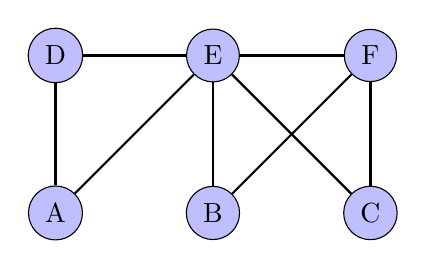
\begin{tikzpicture}
	[node/.style={circle,draw,fill=blue!25!white,minimum size=0.5cm},>=latex]
    \node[node] (A) at (0,0) {A};
    \node[node] (B) at (2,0) {B};
    \node[node] (C) at (4,0) {C};
    \node[node] (D) at (0,2) {D};
    \node[node] (E) at (2,2) {E};
    \node[node] (F) at (4,2) {F};
    \draw [thick] (A) -- (D);
    \draw [thick] (A) -- (E);
    \draw [thick] (B) -- (E);
    \draw [thick] (B) -- (F);
    \draw [thick] (C) -- (E);
    \draw [thick] (C) -- (F);
    \draw [thick] (D) -- (E);
    \draw [thick] (E) -- (F);
\end{tikzpicture}}\hfil
\subfloat[Grafo orientato\label{fig:graph_2}]{
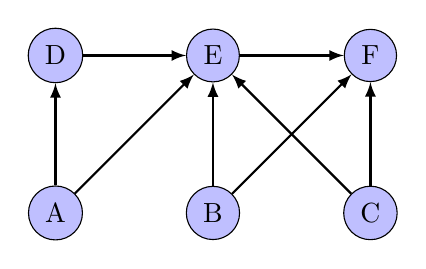
\begin{tikzpicture}
	[node/.style={circle,draw,fill=blue!25!white,minimum size=0.5cm},>=latex]
    \node[node] (A) at (0,0) {A};
    \node[node] (B) at (2,0) {B};
    \node[node] (C) at (4,0) {C};
    \node[node] (D) at (0,2) {D};
    \node[node] (E) at (2,2) {E};
    \node[node] (F) at (4,2) {F};
    \draw [thick,->] (A) -- (D);
    \draw [thick,->] (A) -- (E);
    \draw [thick,->] (B) -- (E);
    \draw [thick,->] (B) -- (F);
    \draw [thick,->] (C) -- (E);
    \draw [thick,->] (C) -- (F);
    \draw [thick,->] (D) -- (E);
    \draw [thick,->] (E) -- (F);
\end{tikzpicture}}
\caption{}
\end{figure}


\begin{osservation}
	    Sia $G=(V,E)$ un grafo, chiaramente il numero massimo di archi possibili sarà: \[|E| \leq |V| \times |V| = |V|^2\] Inoltre, se il grafo è non orientato, allora \[|E| \leq \frac{|V| \times (|V| - 1)}{2} = \binom{|V|}{2}\] Infatti, se il grafo è non orientato, allora: \[(u, v) \in E \iff (v, u) \in E\]
\end{osservation}

Molte definizioni per i grafi orientati e non orientati sono simili, sebbene alcuni termini abbiano significati leggermente diversi nei due contesti.

\dfn{Archi entranti, uscenti ed incidenti}{
    Se $(u,v)$ è un arco in un grafo orientato $G=(V,E)$, diciamo che $(u,v)$ \textbf{esce} dal vertice $u$ ed \textbf{entra} nel vertice $v$. Se $(u,v)$ è un arco in un grafo non orientato, diciamo che $(u,v)$ è \textbf{incidente} nei vertici $u$ e $v$.
}

\begin{figure}[ht!]
\centering
\subfloat[Grafo orientato\label{fig:graph_3}]{
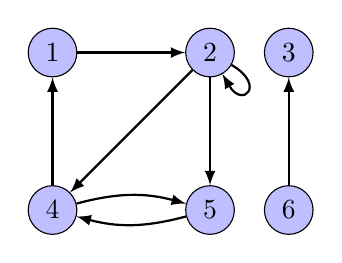
\begin{tikzpicture}
	[node/.style={circle,draw,fill=blue!25!white,minimum size=0.5cm},>=latex]
    \node[node] (A) at (0,0) {4};
    \node[node] (B) at (2,0) {5};
    \node[node] (C) at (3,0) {6};
    \node[node] (D) at (0,2) {1};
    \node[node] (E) at (2,2) {2};
    \node[node] (F) at (3,2) {3};

    \draw[thick,->] (D) -- (E);
    \draw[thick,->] (E) -- (B);
    \draw[thick,->] (E) -- (A);
    \draw[thick,->] (A) -- (D);
    \draw[thick,->] (A) to [bend left = 15] (B);
    \draw[thick,->] (B) to [bend left = 15] (A);
    \draw[thick,->] (C) -- (F);
    \draw[thick,->] (E) to [out=330,in=300,looseness=8] (E);

\end{tikzpicture}
} \hfil
\subfloat[Grafo non orientato\label{fig:graph_4}]{
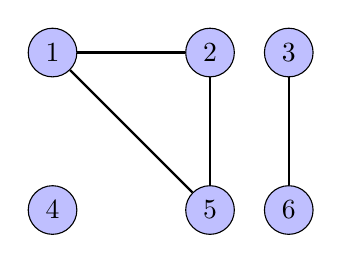
\begin{tikzpicture}
	[node/.style={circle,draw,fill=blue!25!white,minimum size=0.5cm}]
    \node[node] (A) at (0,0) {4};
    \node[node] (B) at (2,0) {5};
    \node[node] (C) at (3,0) {6};
    \node[node] (D) at (0,2) {1};
    \node[node] (E) at (2,2) {2};
    \node[node] (F) at (3,2) {3};

    \draw[thick] (D) -- (E);
    \draw[thick] (E) -- (B);
    \draw[thick] (B) -- (D);
    \draw[thick] (F) -- (C);

\end{tikzpicture}}
\caption{}
\end{figure}


\begin{osservation}
	    In Figura~\ref{fig:graph_3} il vertice $2$ ha due archi entranti e tre archi uscenti. In particolare, un arco che esce ed entra nello stesso vertice viene chiamato \textbf{cappio}. In Figura~\ref{fig:graph_4} il vertice $2$ ha due archi incidenti: $(1,2)$ e $(2,5)$. In un grafo non orientato non è possibile avere cappi.
\end{osservation}

\dfn{Relazione di adiacenza}{
	Se $(u,v)$ è un arco di un grafo $G=(V,E)$, diciamo che il vertice $v$ è \textbf{adiacente} al vertice $u$.
}

Se il grafo non è orientato, la relazione di adiacenza è simmetrica. Se il grafo è orientato, la relazione di adiacenza non è necessariamente simmetrica.


\begin{osservation}
		In Figura~\ref{fig:graph_3} e \ref{fig:graph_4} il vertice $2$ è adiacente al vertice 1, perché l'arco $(1,2)$ appartiene ad entrambi i grafi. Il vertice $1$ non è adiacente al vertice 2 nel grafo mostrato nella Figura~\ref{fig:graph_3} perché l'arco $(2,1)$ non appartiene al grafo.
\end{osservation}

\dfn{Grado di un vertice}{
	Il \textbf{grado} di un vertice in un grafo non orientato è il numero di archi che incidono nel vertice. Un vertice il cui grado è 0 si dice \textbf{isolato}. In un grafo orientato, il \textbf{grado uscente} di un vertice è il numero di archi che escono dal vertice; il \textbf{grado entrante} di un vertice è il numero di archi che entrano nel vertice. Il \textbf{grado} di un vertice in un grafo orientato è la somma del suo grado entrante e del suo grado uscente.
}


\begin{osservation}
		Il vertice 2 nella Figura \ref{fig:graph_4} ha grado 2 mentre il vertice 4 è isolato. Nel grafo in Figura \ref{fig:graph_3} il vertice 2 ha grado entrante 2, grado uscente 3 e grado 5.
\end{osservation}

\subsection{Percorsi in un grafo}\label{sez:grafi_def}

\dfn{Percorso in un grafo}{
	Un \textbf{percorso} di \textbf{lunghezza} $k$ da un vertice $u$ ad un vertice $u'$ in un grafo $G = (V,E)$ è una sequenza di vertici $\langle v_{0},v_{1}, \ldots, v_{k}\rangle$ tali che \[\begin{array}{l}
		u=v_{0} \\  u'=v_{k}
	\end{array}\] e \[\forall i=1,2,\ldots,k \qquad (v_{i-1},v_{i})\in E\]
	La  \textbf{lunghezza} del percorso, o \textbf{cammino}, è il numero di archi presenti nel cammino. Il cammino \textbf{contiene} i vertici $v_{0},v_{1}, \ldots, v_{k}$ e gli archi $(v_{0},v_{1}), (v_{1},v_{2}),\ldots,(v_{k-1},v_{k})$ (c'è sempre un cammino di lunghezza 0 da $u$ ad $u$). Se c'è un cammino $p$ da $u$ ad $u'$, diciamo che $u'$ è \textbf{raggiungibile} da $u$ attraverso $p$ e si denota con il simbolo $u' \leadsto u$. Un cammino si dice \textbf{semplice} se tutti i vertici nel cammino sono distinti.
}


\begin{osservation}
		Nella Figura~\ref{fig:graph_3}, il cammino $\langle 1,2,5,4 \rangle$ è un cammino semplice di lunghezza 3. Il cammino $\langle 2,5,4,5 \rangle$ invece non è semplice.
\end{osservation}

\dfn{Sottopercorso in un grafo}{
	Un \textbf{sottopercorso} di un percorso $p = \langle v_{0},v_{1},\ldots,v_{k}\rangle$ è una sottosequenza contigua dei suoi vertici. Ovvero, per ogni $0 \leq i \leq j \leq k$, la sottosequenza dei vertici $\langle v_{i},v_{i+1},\ldots,v_{k} \rangle$ è un sottopercorso di $p$.
}


\begin{osservation}
		Se la lunghezza di un percorso semplice è limitata dal numero di vertici presenti in un grafo, ovvero $|V|$, il numero di percorsi semplici in un grafo sarà anch'esso limitato in quanto queste saranno tutte e sole le sequenze di lunghezza minore od uguale della cardinalità di $V$.
\end{osservation}

\dfn{Ciclo}{
	In un grafo orientato un cammino $\langle v_{0},v_{1},\ldots,v_{k} \rangle$ forma un \textbf{ciclo} se $v_{0}=v_{k}$ e il cammino contiene almeno un arco. Il ciclo è \textbf{semplice} se $v_{1},...,v_{k}$ sono anche distinti. Un cappio è un ciclo di lunghezza 1. Un grafo orientato senza cappi si dice \textbf{semplice}. In un grafo non orientato un cammino $\langle v_{0},v_{1},\ldots,v_{k} \rangle$ forma un \textbf{ciclo (semplice)} se $k\geq 3,\; v_{0}=v_{k}$ e $v_{1},\ldots,v_{k}$ sono distinti. Un grafo senza cicli è detto \textbf{aciclico}.
}

\begin{figure}[ht!]
	\centering
	\subfloat[Grafo non connesso]{
		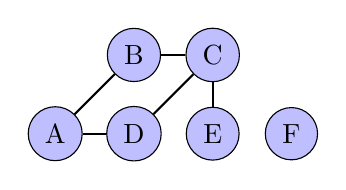
\begin{tikzpicture}
			[node/.style={circle,draw,fill=blue!25!white,minimum size=0.5cm}]
			\node[node] (A) at (0,1) {A};
			\node[node] (B) at (1,2) {B};
			\node[node] (C) at (2,2) {C};
			\node[node] (D) at (1,1) {D};
			\node[node] (E) at (2,1) {E};
			\node[node] (F) at (3,1) {F};

			\draw[thick] (A) -- (B);
			\draw[thick] (A) -- (D);
			\draw[thick] (B) -- (C);
			\draw[thick] (C) -- (D);
			\draw[thick] (C) -- (E);
		\end{tikzpicture}
	} \hfil
	\subfloat[Grafo connesso]{
		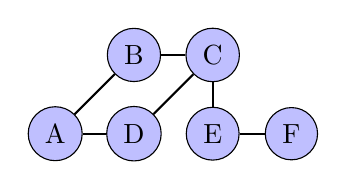
\begin{tikzpicture}
			[node/.style={circle,draw,fill=blue!25!white,minimum size=0.5cm}]

			\node[node] (A) at (0,1) {A};
			\node[node] (B) at (1,2) {B};
			\node[node] (C) at (2,2) {C};
			\node[node] (D) at (1,1) {D};
			\node[node] (E) at (2,1) {E};
			\node[node] (F) at (3,1) {F};

			\draw[thick] (A) -- (B);
			\draw[thick] (A) -- (D);
			\draw[thick] (B) -- (C);
			\draw[thick] (C) -- (D);
			\draw[thick] (C) -- (E);
			\draw[thick] (E) -- (F);
		\end{tikzpicture}
	}
	\caption{}
\end{figure}

Alcuni tipi di grafi hanno dei nomi speciali. Un \textbf{grafo completo} è un grafo non orientato in cui ogni coppia di vertici è adiacente. Un grafo aciclico e non orientato è una \textbf{foresta}; un grafo connesso, aciclico e non orientato è detto \textbf{albero libero}.


\begin{osservation}
		Gli alberi binari studiati nel capitolo 3 non sono altro che particolari tipi di grafi connessi, aciclici e non orientati in cui uno dei vertici si distingue da tutti gli altri, la radice, ed ogni vertice ha un grado entrante pari ad uno ed un grado uscente pari al massimo di due.
\end{osservation}

\section{Rappresentazione dei grafi}
Ci sono due metodi standard per la rappresentazione di un grafo $G=(V,E)$:
\begin{enumerate}
	\item come una collezione di \textbf{liste di adiacenza};
	\item come una \textbf{matrice di adiacenza}.
\end{enumerate}

Entrambi i metodi possono essere applicati sia ai grafi orientati che a quelli non orientati. Di solito, si preferisce la rappresentazione con liste di adiacenza, perché permette di rappresentare in modo compatto i grafi sparsi e richiede una minore occupazione di memoria al variare dei vertici del grafo.\footnote{Una matrice richiederebbe un costo spaziale quadratico sul numero di vertici ($|V|^{2}$) mentre la rappresentazione attraverso liste di adiacenza solo un costo lineare ($|V|$).}

\subsection{Le liste di adiacenza}
La \textbf{rappresentazione con liste di adiacenza} di un grafo $G=(V,E)$ consiste in un array $Adj$ di $|V|$ liste, una per ogni vertice in $V$. Per ogni $u \in V$, la lista di adiacenza $Adj[u]$ contiene tutti i vertici $v$ tali che esista un arco $(u,v)\in E$. Ovvero $Adj[u]$ include tutti i vertici \textbf{adiacenti} ad $u$ in $G$.

Le liste di adiacenza (vedi Figura \ref{fig:lista_adiacenza}) possono essere facilmente adattate per rappresentare i \textbf{grafi pesati}, cioè i grafi per i quali ogni arco ha un \textbf{peso} associato. In questi casi, il peso $w(u,v)$ dell'arco $(u,v) \in E$ viene memorizzato semplicemente assieme al vertice $v$ nella lista di adiacenza di $u$.

\subsection{Le matrici di adiacenza}
Uno svantaggio potenziale della rappresentazione con liste di adiacenza è che non c'è modo più veloce per determinare se un particolare arco $(u,v)$ è presente nel grafo invece che scorrere la lista $Adj[u]$. Per porre un rimedio a questo svantaggio, si può rappresentare il grafo con una \textbf{matrice di adiacenza}, al costo di usare una maggiore quantità di memoria.

Per la \textbf{rappresentazione con matrice di adiacenza} (vedi Figura \ref{fig:matrice_adiacenza}) di un grafo $G=(V,E)$ si suppone che i vertici siano numerati $1,2,\ldots,|V|$ in modo arbitrario. La rappresentazione con matrice di adiacenza di un grafo $G$ consiste in una matrice $A=(a_{ij})$ di dimensioni $|V| \times |V|$ che descrive la \textbf{funzione caratteristica} in $E$:
\begin{equation}
	a_{ij} = \begin{cases}
		1 & \text{se } (i,j)\in E \\
		0 & \text{altrimenti}
	\end{cases}
\end{equation}

\begin{figure}[ht!]
	\centering
	\subfloat[\label{fig:grafo}]
	{
	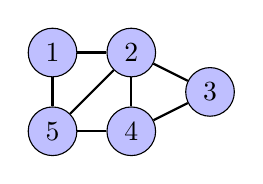
\begin{tikzpicture}
		[node/.style={circle,draw,fill=blue!25!white,minimum size=0.5cm}]
		\node[node,name=1] at (0,1) {1};
		\node[node,name=2] at (1,1) {2};
		\node[node,name=3] at (2,0.5) {3};
		\node[node,name=5] at (0,0) {5};
		\node[node,name=4] at (1,0) {4};
		\draw[thick] (1)--(2);
		\draw[thick] (1)--(5);
		\draw[thick] (2)--(3);
		\draw[thick] (2)--(4);
		\draw[thick] (2)--(5);
		\draw[thick] (3)--(4);
		\draw[thick] (5)--(4);
	\end{tikzpicture}
	} \hfil
	\subfloat[\label{fig:lista_adiacenza}]
	{
	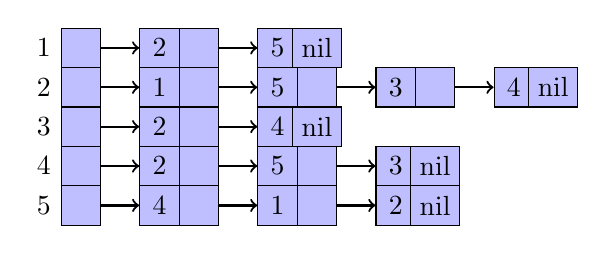
\begin{tikzpicture}
		% draw adjacency list of previous graph
		\node[draw,rectangle,minimum size=0.5cm,fill=blue!25] (1) at (0,1) {};
		\node[draw,rectangle,minimum size=0.5cm,fill=blue!25] (2) at (0,0.5) {};
		\node[draw,rectangle,minimum size=0.5cm,fill=blue!25] (3) at (0,0) {};
		\node[draw,rectangle,minimum size=0.5cm,fill=blue!25] (4) at (0,-0.5) {};
		\node[draw,rectangle,minimum size=0.5cm,fill=blue!25] (5) at (0,-1) {};
		\node[left] at (1.west) {1};
		\node[left] at (2.west) {2};
		\node[left] at (3.west) {3};
		\node[left] at (4.west) {4};
		\node[left] at (5.west) {5};

		\node[draw,rectangle,minimum size=0.5cm,fill=blue!25] (12) at (1,1) {2};
		\node[draw,rectangle,minimum size=0.5cm,fill=blue!25] (121) at (1.5,1) {};
		\node[draw,rectangle,minimum size=0.5cm,fill=blue!25] (15) at (2.5,1) {5};
		\node[draw,rectangle,minimum size=0.5cm,fill=blue!25] (151) at (3,1) {nil};
		\draw[thick,->] (1) -- (12);
		\draw[thick,->] (121) -- (15);

		\node[draw,rectangle,minimum size=0.5cm,fill=blue!25] (21) at (1,0.5) {1};
		\node[draw,rectangle,minimum size=0.5cm,fill=blue!25] (212) at (1.5,0.5) {};
		\node[draw,rectangle,minimum size=0.5cm,fill=blue!25] (22) at (2.5,0.5) {5};
		\node[draw,rectangle,minimum size=0.5cm,fill=blue!25] (221) at (3,0.5) {};
		\node[draw,rectangle,minimum size=0.5cm,fill=blue!25] (23) at (4,0.5) {3};
		\node[draw,rectangle,minimum size=0.5cm,fill=blue!25] (231) at (4.5,0.5) {};
		\node[draw,rectangle,minimum size=0.5cm,fill=blue!25] (24) at (5.5,0.5) {4};
		\node[draw,rectangle,minimum size=0.5cm,fill=blue!25] (241) at (6,0.5) {nil};
		\draw[thick,->] (2) -- (21);
		\draw[thick,->] (212) -- (22);
		\draw[thick,->] (221) -- (23);
		\draw[thick,->] (231) -- (24);

		\node[draw,rectangle,minimum size=0.5cm,fill=blue!25] (31) at (1,0) {2};
		\node[draw,rectangle,minimum size=0.5cm,fill=blue!25] (311) at (1.5,0) {};
		\node[draw,rectangle,minimum size=0.5cm,fill=blue!25] (32) at (2.5,0) {4};
		\node[draw,rectangle,minimum size=0.5cm,fill=blue!25] (321) at (3,0) {nil};
		\draw[thick,->] (3) -- (31);
		\draw[thick,->] (311) -- (32);

		\node[draw,rectangle,minimum size=0.5cm,fill=blue!25] (41) at (1,-0.5) {2};
		\node[draw,rectangle,minimum size=0.5cm,fill=blue!25] (411) at (1.5,-0.5) {};
		\node[draw,rectangle,minimum size=0.5cm,fill=blue!25] (42) at (2.5,-0.5) {5};
		\node[draw,rectangle,minimum size=0.5cm,fill=blue!25] (421) at (3,-0.5) {};
		\node[draw,rectangle,minimum size=0.5cm,fill=blue!25] (43) at (4,-0.5) {3};
		\node[draw,rectangle,minimum size=0.5cm,fill=blue!25] (431) at (4.5,-0.5) {nil};
		\draw[thick,->] (4) -- (41);
		\draw[thick,->] (411) -- (42);
		\draw[thick,->] (421) -- (43);

		\node[draw,rectangle,minimum size=0.5cm,fill=blue!25] (51) at (1,-1) {4};
		\node[draw,rectangle,minimum size=0.5cm,fill=blue!25] (511) at (1.5,-1) {};
		\node[draw,rectangle,minimum size=0.5cm,fill=blue!25] (52) at (2.5,-1) {1};
		\node[draw,rectangle,minimum size=0.5cm,fill=blue!25] (521) at (3,-1) {};
		\node[draw,rectangle,minimum size=0.5cm,fill=blue!25] (53) at (4,-1) {2};
		\node[draw,rectangle,minimum size=0.5cm,fill=blue!25] (531) at (4.5,-1) {nil};
		\draw[thick,->] (5) -- (51);
		\draw[thick,->] (511) -- (52);
		\draw[thick,->] (521) -- (53);
	\end{tikzpicture}
	} \hfil
	\subfloat[\label{fig:matrice_adiacenza}]
	{
	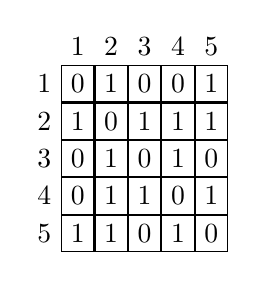
\begin{tikzpicture}[every node/.style=draw]
	\pgfmatrix{rectangle}{center}{mymatrix}
	{\pgfusepath{}}{\pgfpointorigin}{\let\&=\pgfmatrixnextcell}
	{
		\node (a){0}; \& \node(b) {1}; \& \node (c) {0}; \& \node (d) {0}; \& \node (e) {1}; \\
		\node (f){1}; \& \node(g) {0}; \& \node (h) {1}; \& \node (i) {1}; \& \node (l) {1}; \\
		\node (m){0}; \& \node(n) {1}; \& \node (o) {0}; \& \node (p) {1}; \& \node (q) {0}; \\
		\node (r){0}; \& \node(s) {1}; \& \node (t) {1}; \& \node (u) {0}; \& \node (v) {1}; \\
		\node (w){1}; \& \node(x) {1}; \& \node (y) {0}; \& \node (z) {1}; \& \node (aa) {0}; \\
	}
	\node[left,draw=white] at (a.west) {1};
	\node[left,draw=white] at (f.west) {2};
	\node[left,draw=white] at (m.west) {3};
	\node[left,draw=white] at (r.west) {4};
	\node[left,draw=white] at (w.west) {5};
	\node[above,draw=white] at (a.north) {1};
	\node[above,draw=white] at (b.north) {2};
	\node[above,draw=white] at (c.north) {3};
	\node[above,draw=white] at (d.north) {4};
	\node[above,draw=white] at (e.north) {5};
	\end{tikzpicture}
	}
	\caption{Due rappresentazioni di un grafo non orientato. \textbf{(\ref{fig:grafo})} Un grafo non orientato $G$ con cinque vertici e sette archi. \textbf{(\ref{fig:lista_adiacenza})} Una rappresentazione con liste di adiacenza di $G$. \textbf{(\ref{fig:matrice_adiacenza})} Una rappresentazione con matrice di adiacenza di $G$.}
\end{figure}

\section{Visita in ampiezza}
La \textbf{visita in ampiezza} (\textsc{Breadth-First-Search}) è uno dei più semplici algoritmi di ricerca nei grafi e sta alla base di molti algoritmi che operano con i grafi. Dato un grafo $G=(V,E)$ e un vertice distinto $s$, detto \textbf{sorgente}, la visita in ampiezza ispeziona sistematicamente gli archi di $G$ per ``scoprire'' tutti i vertici raggiungibili da $s$ individuando la distanza da $s$ ad ognuno dei vertici raggiungibili. La visita in ampiezza è chiamata così infatti perché espande la frontiera fra i vertici scoperti e quelli da scoprire in maniera uniforme lungo l'ampiezza della frontiera. Questo significa che l'algoritmo scopre tutti i vertici che si trovano ad una distanza $k$ da $s$, prima di scoprire i vertici a distanza $k+1$.

Per tenere traccia del lavoro svolto ed evitare di raggiungere nodi già visitati in precedenza, la visita in ampiezza colora i vertici di bianco, di grigio o di nero:
\begin{itemize}
	\item \textbf{Bianco:} il nodo non è stato ancora visitato;
	\item \textbf{Grigio:} il nodo è stato visitato ma potrebbe avere di vicini non visitati;
	\item \textbf{Nero:} il nodo è stato visitato ed anche tutti i suoi vicini.
\end{itemize}
Inizialmente tutti i vertici sono bianchi; successivamente possono diventare grigi ed infine neri. Per questo motivo possiamo implementare l'algoritmo \textsc{Init(G)} (Algoritmo~\ref{lst:init}) che si occupa di inizializzare un grafo colorando tutti i suoi vertici di bianco.
\begin{lstlisting}[language=asd,caption={Init(G)},label=lst:init]
for each v in V do
	Color[v] = White
\end{lstlisting}

Un vertice viene \textbf{scoperto} quando viene incontrato per la prima volta durante la visita; in quel momento cessa di essere un vertice bianco. Se $(u,v) \in E$ e il vertice $u$ è nero, allora il vertice $v$ è grigio oppure nero: ovvero tutti i vertici adiacenti ai vertici neri sono sempre scoperti. I vertici grigi possono avere qualche vertice bianco adiacente per questo motivo essi rappresentano la frontiera fra i vertici scoperti e quelli da scoprire.

\begin{center}
	\includegraphics{res/dfs_frontiera}
	\captionof{figure}{L'algoritmo di visita in ampiezza estende di volta in volta la frontiera dei vertici da visitare}
\end{center}

La vista in ampiezza costruisce una coda $Q$ che, inizialmente contiene soltanto il vertice sorgente $s$. A questo punto si accodano tutti i vertici presenti colorati di bianco scoperti esplorando la lista di adiacenza e li si colora di grigio. Una volta aver eseguito questa operazione si estrae il nodo in testa alla coda, lo si colora di nero e si aggiungono in coda i  vertici bianchi adiacenti scoperti esplorando la lista di adiacenza. L'algoritmo viene eseguito fino a quando la coda non risulta vuota.


\begin{lstlisting}[language=asd,caption={BFS(G,s)},label=lst:bfs_graph]
Init(G)
Q={s}
Color[s] = Gray
while Q @\neq@ {} do
	x = Head(Q)
	foreach v @\in@ Adj(x) do
		if Color[v] = b then
			Q = Enqueue(Q,v)
			Color[v] = Gray
	Q = Dequeue(Q)
	Color[x] = Black
\end{lstlisting}

\subsection{Una versione migliorata dell'algoritmo BFS}
L'Algoritmo~\ref{lst:bfs_graph} visita i vertici raggiungibili di un grafo al crescere della loro distanza dal vertice sorgente $s$. Ciò significa che ciascun vertice viene raggiunto tramite il cammino più breve possibile da $s$. Infatti, per ogni vertice $v$ raggiungibile da $s$, il cammino semplice che va da $s$ a $v$ corrisponde ad un cammino minimo da $s$ a $v$, cioè un cammino che contiene il minor numero di archi possibile.

\dfn{Distanza di un vertice}{
	La \textbf{distanza} di un vertice $v$ dal vertice sorgente $s$ è il numero di archi nel cammino minimo da $s$ a $v$, e si indica con $d(s,v)$.
}

Osserviamo che l'algoritmo \textsc{BFS} determina una \textit{relazione gerarchica} fra i vertici di un grafo. Infatti, la visita in ampiezza costruisce un albero, detto \textbf{albero breath first (BF)}, che inizialmente contiene soltanto la sua radice, ovvero il vertice sorgente $s$. Quando un vertice bianco $v$ viene scoperto durante l'ispezione della lista di adiacenza di un vertice $u$ già scoperto, il vertice $v$ e l'arco $(u,v)$ vengono aggiunti all'albero. Il vertice $u$ rappresenta così il \textbf{predecessore} o \textbf{padre} di $v$ nell'albero \textsc{BF} e dato che un vertice verrà scoperto sempre e solo una volta, ogni vertice avrà sempre e solo un padre nell'albero \textsc{BF}. È così univocamente determinata la funzione $$p:V \rightarrow \mathbb{N}\cup \{nil\}$$ che associa ad ogni nodo l'indice del vertice padre. A partire da questa osservazione possiamo definire un raffinamento dell'Algoritmo~\ref{lst:bfs_graph} che costruisce l'albero \textsc{BF} a partire dai percorsi minimi da $s$ a tutti i vertici raggiungibili.

L'Algoritmo~\ref{lst:bfs_graph_2} calcola quindi la distanza di ogni vertice raggiungibile da $s$ come il numero di archi nel cammino minimo da $s$ al vertice. Questa quantità è memorizzata nell'array $d$. Chiaramente, la distanza da $s$ a $v$ è data dalla distanza da $s$ al suo predecessore, più 1. Useremo il valore $\infty$ per indicare che un vertice non è raggiungibile da $s$. Oltre al vettore $d$ che memorizza le distanze, l'algoritmo utilizza un vettore $p$ che memorizza i predecessori di ogni vertice nell'albero \textsc{BF}. Il predecessore di un vertice $v$ è il vertice $u$ che ha scoperto $v$ per la prima volta. Il predecessore di $s$ è indicato con il valore $nil$.

\begin{lstlisting}[language=asd,caption={BFS(G,s)},label=lst:bfs_graph_2]
for each x in V do
	Color[x] = white
	d[x]=@$\infty$@
	p[x] = nil
Q={s}
Color[s] = Gray
d[s] = 0
p[s] = nil
while Q @\neq@ {} do
	x = Head(Q)
	foreach v @\in@ Adj(x) do
		if Color[v] = b then
			Q = Enqueue(Q,v)
			Color[v] = Gray
			d[v] = d[x] + 1
			p[v] = x
	Q = Dequeue(Q)
	Color[x] = Black
\end{lstlisting}

\subsection{Correttezza dell'algoritmo BFS}
Prima di dimostrare le varie proprietà della visita in ampiezza, analizziamo il suo tempo di esecuzione con un grafo di input $G=(V,E)$.

Dopo l'inizializzazione, nessun vertice sarà più colorato di bianco, quindi il test nella riga 12 garantisce che ciascun vertice venga accodato al più una volta, e di conseguenza, venga eliminato dalla coda al più una volta. Le operazioni di inserimento e cancellazione dalla coda richiedono un tempo costante, quindi il tempo totale dedicato alle operazioni con la coda risulta lineare sulla dimensione dei vertici del grafo $G$.

Poiché la lista di adiacenza di ciascun vertice viene ispezionata soltanto quando il vertice viene rimosso dalla coda, ogni lista di adiacenza viene ispezionata al più una volta. Poiché l'algoritmo ispeziona le liste di adiacenza di ciascun vertice, la cui somma totale \footnote{Di tutte le liste.}delle lunghezze è pari ad $|E|$, allora il tempo di esecuzione totale di \textsc{BFS} risulta lineare nella dimensione della rappresentazione con liste di adiacenza del grafo $G$: $E+V$.


\begin{teorbox}
	Dato un arbitrario grafo $G$ ed un vertice $s \in V$, al termine dell'esecuzione dell'Algoritmo \textsc{BFS} devono valere:
\begin{enumerate}
	\item $\forall v \in V$, $v$ sarà visitato se e soltato se $v$ è \textit{raggiungibile} da $s$;
	\item $\forall v \in V$ vale: $d[v] = \delta(v,s)$;
	\item $\forall v \in V\setminus\{s\}$, se $v$ è raggiungibile allora è ottenibile un percorso minimo da $s$ a $v$ concatenando il percorso minimo da $s$ a $p[v]$.
\end{enumerate}
\end{teorbox}

Il teorema appena enunciato garantisce la correttezza dell'algoritmo \textsc{BFS}. Al contrario degli algoritmi finora visti, dove si è utilizzato il principio di induzione per dimostrare la correttezza, la dimostrazione della correttezza dell'algoritmo \textsc{BFS} non è così immediata in quanto l'algoritmo è stato definito in maniera iterativa. Per dimostrare quindi tale correttezza bisogna studiare il comportamento del programma durante l'esecuzione e dimostrare che le tre proprietà enunciate dal teorema sono sempre valide. Questa tipologia di analisi prende il nome di \textbf{analisi a invariante}.

\begin{propbox}[Proprietà della funzione $\delta$ o disuguaglianza triangolare]
Per ogni coppia $(u,v)$ di vertici di un grafo $G$, se $(u,v) \in E$ allora $\delta(s,v) \leq \delta(s,u) + 1$ per ogni vertice $s$.
\begin{center}
	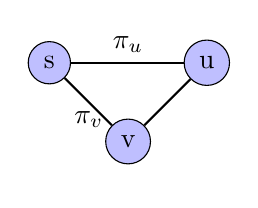
\begin{tikzpicture}
		% draw a graph with three paths and describe the delta function's property
		[node/.style={circle,draw,fill=blue!25!white,minimum size=0.5cm},>=latex]
		\node[node] (u) at (0,0) {s};
		\node[node] (v) at (2,0) {u};
		\node[node] (w) at (1,-1) {v};

		\draw[thick] (u) -- (v);
		\draw[thick] (u) -- (w);
		\draw[thick] (w) -- (v);

		\node[above] at (1,0) {$\pi_{u}$};
		\node[below] at (0.5,-0.5) {$\pi_{v}$};
		\node[below] at (1.5,-0.5) {};

		\node[above] at (1,-1.5) {};
	\end{tikzpicture}
\end{center}
\end{propbox}

\begin{proof}
	Supponiamo che la proprietà sia falsa. Allora esiste una coppia $(u,v)$ di vertici di un grafo $G$ tale che $(u,v) \in E$ e $\delta(s,v) > \delta(s,u) + 1$ per ogni vertice $s$.

Sia $\pi_{u}$ un cammino minimo da $s$ a $u$ e sia $\pi_{v}$ un cammino minimo da $s$ a $v$ e consideriamo il percorso $\pi_{u} \cdot v$. Questo percorso è un cammino da $s$ a $v$ e la sua lunghezza è $\delta(s,u) + 1$. Poiché $\delta(s,v) > \delta(s,u) + 1$, allora $\pi_{u} \cdot v$ è un cammino da $s$ a $v$ più corto di $\pi_{v}$, il che è assurdo perché $\pi_{v}$ è un cammino minimo da $s$ a $v$.
\end{proof}


\begin{propbox}[Proprietà A]
	Durante l'esecuzione di \textsc{BFS}$(G,s)$, per ogni vertice $v \in V$ si ha:
	\begin{displaymath}
		d[v] \geq \delta(s,v)
	\end{displaymath}
\end{propbox}
\begin{proof}
	Per dimostrare l'invarianza della proprietà A si procede per induzione sul numero di accodamenti in $Q$. Questo perché le modifiche ai valori di $d[v]$ avvengono soltanto in corrispondenza degli accodamenti dei vertici in $Q$. Tutto ciò che non è un accodamento, infatti, non modifica i valori di $d[v]$. Indichiamo tale numero con $k$:
\begin{enumerate}
	\item \textbf{Caso base:} Sia $k=0$. All'inizio dell'esecuzione di \textsc{BFS}$(G,s)$, $Q$ contiene soltanto il vertice $s$. Poiché $d[s]=0$ e $\delta(s,s)=0$, la proprietà A è verificata.
	\item \textbf{Caso induttivo:} Sia $k>1$ e assumiamo che la proprietà sia verificata per $k-1$ accodamenti. Tra il $k-1$-esimo ed il $k$-esimo accodamento non avviene alcuna modifica ai valori di $d$. Sia $x$ l'ultimo vertice accodato e supponiamo di eseguire l'accodamento di un vertice $v$. Essendo $x$ già presente nella coda la sua distanza è stata già calcolata e vale, per ipotesi induttiva:
	\[d[x] \geq \delta(s,x)\]
	Maggiorando entrambi i membri della disuguaglianza triangolare con $+1$ si ottiene:
	\[d[x]+1 \geq \delta(s,x)+1\]
	Dovendo accodare $v$ si presuppone che esista un arco che vada da $x$ a $v$, ovvero $(x,v) \in E$. Per la proprietà della funzione $\delta$ si ha allora:
	\[\delta(s,x) + 1 \geq \delta(s,v) \]
	Per transitività si ottiene:
	\[d[x]+1 \geq \delta(s,v)\]
	Per la definizione di $d[v]$ si ha quindi l'enunciato:
	\[d[v] \geq \delta(s,v)\]
\end{enumerate}
\end{proof}

Una seconda proprietà invariante che andiamo a dimostrare descrive la relazione fra le stime delle distanze dei vertici accodati.

\begin{propbox}[Proprietà B]
	Durante l'esecuzione di \textsc{BFS}$(G,s)$, se $Q=\langle v_{1},v_{2},\ldots,v_{k}\rangle$ allora valgono le seguenti proprietà:
	\begin{enumerate}
		\item $d[v_{k}] \leq d[v_{1}]+1$;
		\item $d[v_{i}] \leq d[v_{i+1}]$ per $i=1,2,\ldots,k-1$.
	\end{enumerate}
\end{propbox}
\begin{proof}
	Come già osservato in precedenza, le stime delle distanze vengono modificate soltanto in corrispondenza delle operazioni eseguite sulla coda $Q$, per questo motivo bisogna tenere in considerazione tutte le operazioni di accodamento e decodamento. Sia $k$ il numero di tali operazioni e procediamo per induzione su $k$:
\begin{itemize}
	\item \textbf{Caso base:} Sia $k=0$. All'inizio dell'esecuzione di \textsc{BFS}$(G,s)$, $Q$ contiene soltanto il vertice $s$. Poiché $d[s]=0$ le due proprietà sono banalmente verificate.
	\item \textbf{Caso induttivo:} Sia $k>1$, bisogna dimostrare che la proprietà sia valida dopo l'inserimento e la rimozione di un vertice nella coda. Se il vertice $v_{1}$ viene eliminato dalla coda, il vertice $v_{2}$ diventa la nuova testa (se la coda si svuota, allora ci troviamo nuovamente nel caso base). Per l'ipotesi induttiva si ha:
	\[d[v_{1}] \leq d[v_{2}]\]
	ma allora si ha:
	\[d[v_{k}]\leq d[v_{1}]+1 \leq d[v_{2}]+1\]
	e le restanti disuguaglianze restano inalterate. L'inserimento di un nuovo vertice richiede invece un esame più attento del codice. Quando inseriamo nella coda un vertice $v$, questo diventa l'ultimo elemento della coda, ovvero $v_{k+1}$ e si pone:
	\[d[v_{k+1}] = d[x]+1\]
	dove $x$ rappresenta la testa della coda prima dell'inserimento di $v$,	il che dimostra la prima proprietà. Per la seconda proprietà bisogna dimostrare che:
	\[ d[v_{k}] \leq d[v_{k+1}] \]
	Chiaramente, prima dell'accodamento del vertice $v$ valeva la seguente relazione per vertice $v_{k}$:
	\[ d[v_{k}] \leq d[v_{1}]+1 = d[v_{k+1}] \]
	che è la tesi della seconda proprietà.
\end{itemize}
\end{proof}

\begin{propbox}[Proprietà C]
	È possibile partizionare l'insieme dei vertici $V$ in varie partizioni $V_{0},V_{1},\ldots,V_{k}$ tali che:
	\begin{itemize}
		\item $V_{0} = \{s\}$;
		\item $V_{1}$ contiene i vertici adiacenti di $s$ meno $s$ stesso;
		\item $V_{2}$ contiene i vertici adiacenti di $V_{i-1}$ meno i vertici già presenti in $V_{0},V_{1}$.
		\item $V_{i}$ contiene i vertici adiacenti di $V_{i-1}$ meno i vertici già presenti in $V_{0},V_{1},\ldots,V_{i-1}$.
		\item $V_{\infty}$ contiene i vertici non raggiungibili da $s$.
	\end{itemize}
\end{propbox}

Si osserva che un vertice non raggiungibile $v$ non può mai essere accodato. Infatti, se per assurdo si suppone che $v$ sia il primo vertice non raggiungibile ad essere accodato, allora deve esistere un vertice $x \in Q$ per cui $(x,v) \in E$. Essendo $x$ un vertice raggiungibile allora esiste sicuramente un percorso dalla sorgente al vertice $v$ che passa per $x$. Ma allora $v$ è raggiungibile, il che è assurdo. Quindi, se $v$ non è raggiungibile, allora $v$ non può essere accodato. Grazie a questa osservazione è possibile dimostrare la correttezza dell'algoritmo \textsc{BFS} semplicemente dimostrando il seguente lemma.

\begin{lemmabox}
	Per ogni $i \in \mathbb{N}$, per ogni vertice $v \in V_{i}$ vale che esiste un unico istante durante l'esecuzione dell'algoritmo \textsc{BFS} tale per cui:
	\begin{enumerate}
		\item $v$ viene colorato di grigio e aggiunto alla coda $Q$;
		\item $d[v] = i$;
		\item il predecessore di $v$ è impostato ad un vertice $u \in V_{i-1}$ e $(p[v],v) \in E$ con $v \neq s$.
	\end{enumerate}
\end{lemmabox}
\begin{proof}
	Si dimostra per induzione su $i$:
\begin{enumerate}
	\item \textbf{Caso base:} $i=0$ e $v=s$. All'inizio dell'esecuzione di \textsc{BFS}$(G,s)$, $Q$ contiene soltanto il vertice $s$ e le tre proprietà sono banalmente vere.
	\item \textbf{Caso induttivo:} sia $i>0$ e si supponga il lemma vero per $V_{j}$ con $j<i$. Se $v \in V_{i}$ arbitrario allora esiste per forza un momento in cui questo verrà colorato di grigio ed accodato. Ciò significa che esiste un percorso da $s$ a $v$ che passa per un vertice $x$ che è stato accodato al più $i-1$-esimo accodamento. Quindi, $x \in V_{i-1}$. Per ipotesi induttiva allora $d[x] = i-1$ e $p[x] \in V_{i-2}$. Poiché $x$ è stato accodato al più $i-1$-esimo accodamento, allora $v$ è stato accodato al $i$-esimo accodamento. Quindi, $d[v] = d[x]+1 = (i-1)+1 = i$ e $p[v] = x$.
\end{enumerate}
\end{proof}

\section{Visita in profondità}
A differenza della visita in ampiezza che si propone di visitare un grafo per distanze crescenti, la visita in profondità (\textsc{Depth-First-Search}) si propone di visitare un grafo esplorando tutti i nodi visitabili lungo i vari percorsi che si diramano a partire da un nodo sorgente $s$.

La visita in profondità è stata già descritta in relazione alle strutture dati ramificate come gli alberi dove, a differenza dei grafi, è implicita nella struttura il concetto di \textit{figlio sinistro} e \textit{figlio destro}. In un grafo, invece, non esiste alcuna relazione gerarchica tra i vari nodi e sarà quindi necessario adottare una strategia diversa da quella utilizzata per la visita in ampiezza che faceva uso di una coda per memorizzare i nodi da visitare.

Nella visita in profondità, ci avvaleremo di quattro array ausiliari per memorizzare lo stato dei nodi del grafo:
\begin{enumerate}
	\item \texttt{Color[]} che memorizza lo stato dei nodi codificati per colore: \texttt{White} se il nodo non è stato ancora visitato, \texttt{Gray} se il nodo è stato visitato ma non tutti i suoi vicini sono stati visitati, \texttt{Black} se il nodo è stato visitato e tutti i suoi vicini sono stati visitati;
	\item \texttt{d[]} che memorizza il tempo di scoperta di un nodo;
	\item \texttt{f[]} che memorizza il tempo di completamento di un nodo;
	\item \texttt{p[]} che memorizza il predecessore di un nodo.
\end{enumerate}
Per memorizzare i vari istanti di tempo assumiamo di dichiarare una variabile globale \texttt{time} che verrà incrementata ad ogni chiamata ricorsiva della funzione \textsc{DFS-Visit}. Si hanno quindi i seguenti algoritmi: \texttt{Init(G)}, \texttt{DFS(G)} e \texttt{DFS-Visit(G,u)}. L'algoritmo \texttt{Init(G)} inizializza gli array ausiliari \texttt{pred[]} e \texttt{color[]}, mentre l'algoritmo \texttt{DFS(G)} esegue la visita in profondità del grafo $G$ richiamando la funzione \texttt{DFS-Visit(G,u)} per ogni nodo $u \in V$ che non è ancora stato visitato.
\begin{center}
\begin{minipage}{,4\textwidth}
\begin{lstlisting}[language=asd,caption={Init(G)},label=lst:init_graph]
for each v @$\in$@ V do
	Color[v] = White
	Pred[v] = nil
time = 1
\end{lstlisting}
\end{minipage}
\begin{minipage}{0.4\textwidth}
	\begin{lstlisting}[language=asd,caption={DFS(G)},label=lst:dfs_graph]
	Init(G)
	for each v @$\in$@ V do
		if Color[v] = White then
			DFS-Visit(G,v)
	\end{lstlisting}
\end{minipage}
\end{center}
\begin{lstlisting}[language=asd,caption={DFS-Visit(G,s)},label=lst:dfs_visit_graph]
Color[s] = Gray
time = time+1
d[s] = time
for each v @$\in$@ Adj(s) do
	if Color[v] = White then
		Pred[v] = s
		DFS-Visit(G,v)
time = time+1
f[s] = time
Color[s] = Black
\end{lstlisting}

\begin{center}
	\includegraphics[scale=0.55]{res/DFS_forest}
	\captionof{figure}{Foresta generata dalla visita in profondità di un grafo.}\label{fig:fdf}
\end{center}

Come nella visita in ampiezza, quando un vertice $v$ viene scoperto durante un'ispezione della lista di adiacenza di un vertice $s$ già scoperto, la visita in profondità registra questo evento assegnando $pred[v]=s$. Diversamente dalla visita in ampiezza però, dove l'ispezione delle liste di adiacenza produceva un albero dei predecessori (l'albero BF), la visita in profondità genera una foresta di alberi, detta \textbf{foresta depth first (DF)} (vedi Figura \ref{fig:fdf}), che è composta da vari \textbf{alberi depth first (DF)} in quanto la visita può essere ripetuta da più sorgenti. L'albero DF di un vertice $s$ è composto da tutti i vertici raggiungibili da $s$ e da tutti gli archi $(s,v)$ tali che $v$ è il primo vertice scoperto durante la visita di $s$.

Volendo fare una analisi del tempo di esecuzione dell'algoritmo \textsc{DFS} si osserva che ciascuna chiamata ricorsiva della funzione \textsc{DFS-Visit} richiede un tempo costante per inizializzare il colore del vertice $u$ e un tempo lineare sulla dimensione della lista di adiacenza di $u$ per ispezionarla completamente. Poiché la somma delle lunghezze di tutte le liste di adiacenza è pari a $|E|$, il tempo totale richiesto per ispezionare tutte le liste di adiacenza è lineare su tale grandezza. Inoltre, poiché ogni vertice viene visitato una sola volta, si avrà che il numero totale di chiamate sia lineare sul numero dei vertici del grafo. Quindi, il tempo totale richiesto per eseguire la visita in profondità di un grafo $G=(V,E)$ è pari a $|V|+|E|$.


\begin{osservation}
		La visita in profondità non garantisce la scoperta dei percorsi minimi da $s$ a tutti i vertici raggiungibili. Infatti, il percorso seguito dall'algoritmo dipende dalla scelta dell'ordine in cui vengono esplorati i vertici nelle liste di adiacenza. Al contrario, la visita in ampiezza garantisce la scoperta dei percorsi minimi da $s$ a tutti i vertici raggiungibili in quanto questa procede in maniera sistematica seguendo distanze progressive.
\end{osservation}

\subsection{Proprietà della visita in profondità}\label{sez:prop_dfs}
Come già detto in precedenza, la visita in profondità genera un \textbf{sottografo dei predecessori} $G'$ che prende il nome di \textbf{foresta depth first}. Poniamo $G'$ come segue:
\begin{displaymath}
	\begin{array}{l}
		G' = (V', E') \\
		V' = V \\
		E' = \{(p[v],v):v \in V \setminus \{s\} \land p[v] \neq nil\}\\
	\end{array}
\end{displaymath}
Come nella visita in ampiezza, i vertici vengono colorati durante la visita in profondità per indicare il loro stato. Inizialmente tutti i vertici sono bianchi. Un vertice diventa grigio quando viene \textbf{scoperto} durante la visita; diventa nero quando viene \textbf{completato}, ovvero quando la sua lista di adiacenza è stata completamente ispezionata. Questa tecnica garantisce che ogni vertice vada a finire in un solo albero DF, in modo che questi alberi siano disgiunti.

Va notato inoltre che la struttura ad albero di un albero DF è determinata dalla sequenza di chiamate ricorsive di \textsc{DFS-Visit}. Infatti, ogni volta che viene scoperto un vertice $v$ durante la visita di un vertice $u$, il vertice $v$ diventa un figlio di $u$ nell'albero DF. Inoltre, il vertice $u$ diventa il predecessore di $v$ nell'albero DF. Per questo motivo, la struttura della foresta DF rispecchia esattamente la struttura delle chiamate ricorsive di \textsc{DFS-Visit}.

Un'altra importante proprietà della visita in profondità è che i tempi di scoperta e completamento hanno una \textbf{struttura di parentesi}. Se rappresentiamo la scoperta del vertice $u$ con una parentesi aperta ``$(u$'' e il suo completamento con una parentesi chiusa ``$u)$'', allora la storia delle scoperte e dei completamenti produce un'espressione ben formata, nel senso che le parentesi sono opportunamente annidate.


\begin{teorbox}
	Dato $G=(V,E)$, al termine di \textsc{DFS}$(G)$, per ogni coppia di vertici $u$ e $v$ vale una delle seguenti condizioni:
	\begin{enumerate}
		\item $d[v] < d[u] < f[u] < f[v]$;
		\item $d[u] < d[v] < f[v] < f[u]$;
		\item $d[v] < f[v] < d[u] < f[u]$;
		\item $d[u] < f[u] < d[v] < f[v]$;
	\end{enumerate}
\end{teorbox}

\begin{proof}
Dimostriamo il teorema mostrando che la condizione $d[v]<d[u]<f[v]<f[u]$ non può mai verificarsi. Ragioniamo quindi per assurdo ed ipotizziamo che tale condizione possa verificarsi. Per questo motivo esisterà un momento nell'esecuzione dell'algoritmo in cui verrà assegnato il tempo $d[v]$.

Consideriamo quindi uno stack sul quale vengono inseriti i vari record di attivazione per ciascuna chiamata di \textsc{DFS-Visit}. Quando viene eseguita la chiamata \textsc{DFS-Visit}$(G,v)$, ovvero nell'istante $d[v]$ il record di attivazione per la chiamata viene inserito in cima alla pila:
\begin{center}
	%\includegraphics[scale=0.5]{res/Struttura_Parentesi1}
	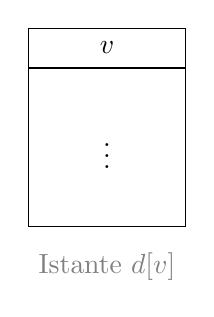
\begin{tikzpicture}
		\node[rectangle,draw=black,minimum width=2cm,minimum height=2cm](stack){$\vdots$};
		\node[rectangle,draw=black,minimum width=2cm,minimum height=0.5cm,anchor=south] at (stack.north) {$v$};
		\node[gray,yshift=-0.5cm]at (stack.south) {Istante $d[v]$};
	\end{tikzpicture}
\end{center}
Più avanti con le chiamate si arriva all'istante $d[u]$ e il record di attivazione della chiamata \textsc{DFS-Visit}$(G,u)$ viene inserito in cima alla pila:
\begin{center}
	%\includegraphics[scale=0.5]{res/Struttura_Parentesi1}
	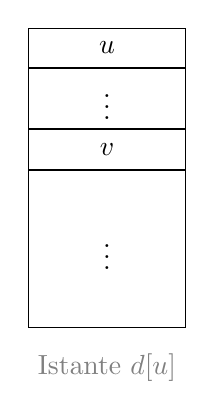
\begin{tikzpicture}
		\node[rectangle,draw=black,minimum width=2cm,minimum height=2cm](stack){$\vdots$};
		\node[rectangle,draw=black,minimum width=2cm,minimum height=0.5cm,anchor=south](v) at (stack.north) {$v$};
		\node[rectangle,draw=black,minimum width=2cm,minimum height=0.5cm,anchor=south](d) at (v.north) {$\vdots$};
		\node[rectangle,draw=black,minimum width=2cm,minimum height=0.5cm,anchor=south](u) at (d.north) {$u$};
		\node[gray,yshift=-0.5cm]at (stack.south) {Istante $d[u]$};
	\end{tikzpicture}
\end{center}
A questo punto si dovrebbe assegnare l'algoritmo di fine visita del vertice $v$ e per farlo si dovrebbe avere il record della chiamata \textsc{DFS-Visit}$(G,v)$ in cima allo stack ma al suo posto c'è il record del vertice $u$. Per terminare $v$ quindi si potrebbe pensare o di aggiungere un nuovo record per \textsc{DFS-Visit}$(G,v)$ in cima allo stack oppure di rimuovere il record del vertice $u$. Entrambe le soluzioni, però, non sono ammesse in quanto, come sappiamo, ogni vertice entra nello stack una ed una sola volta ed inoltre, per rimuovere il record del vertice $u$ andrebbe prima assegnato il suo tempo di completamento (ci troviamo ancora in un istante compreso tra $d[u]$ ed $f[u]$). Per questo motivo questa sequenza è impossibile da ottenere.
\end{proof}

\begin{corolbox}[Annidamento degli intervalli dei discendenti]
	Per ogni vertice $u,v \in V$, il vertice $u$ è discendente di $v$ nella foresta DF se e soltanto se:
	\begin{equation}\label{eq:condizione_discendenza}
		d[v]<d[u]<f[u]<f[v]
	\end{equation}
\end{corolbox}
\begin{proof}
	Siano $v$ e $z$ due vertici di $V$ si supponga di avere la seguente condizione sullo stack:
\begin{center}
	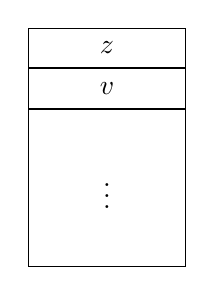
\begin{tikzpicture}
		\node[rectangle,draw=black,minimum width=2cm,minimum height=2cm](stack){$\vdots$};
		\node[rectangle,draw=black,minimum width=2cm,minimum height=0.5cm,anchor=south](v) at (stack.north) {$v$};
		\node[rectangle,draw=black,minimum width=2cm,minimum height=0.5cm,anchor=south](u) at (v.north) {$z$};
	\end{tikzpicture}
\end{center}
Ciò significa che la chiamata a \textsc{DFS-Visit}$(G,v)$ ha generato la chiamata sul vertice $z$. Allora esisterà sicuramente un arco $(v,z) \in E$ che corrisponderà ad un arco nel sottografo dei predecessori. Allora sicuramente $p[z] = v$. Dato lo stack di attivazione possiamo mappare quindi ogni sequenza di vertici con una sequenza nella foresta depth first. In questo modo si dimostra che la condizione è sufficiente.

Sia ora $u$ discendente di $v$ nella foresta depth first e ragioniamo per induzione sulla lunghezza del percorso $\pi$ da $v$ ad $u$:
\begin{itemize}
	\item \textbf{Caso base:} sia $|\pi|=1$ allora esiste un solo arco tra $v$ ed $u$ e $p[u]=v$. Se $p[u]=v$ allora sicuramente si avrà la sequenza $d[v]<d[u]<f[u]<f[v]$ per il teorema della struttura parentesi.
	\item \textbf{Caso induttivo:} sia $|\pi|>1$ e sia l'implicazione valida per $|\pi| -1$. Possiamo decomporre $\pi$ in due parti: $$\pi = \underbrace{\langle v \ldots z \rangle}_{\pi'} + \langle z,u \rangle$$
	Chiaramente $\pi'$ ha lunghezza $|\pi|-1$, quindi per ipotesi induttiva vale $d[v]<d[z]<f[z]<f[v]$. Resta da capire dove si collocano gli istanti $d[u]$ e $f[u]$ all'interno di tale sequenza. Osserviamo però che l'arco $\langle z,u \rangle$ ha dimensione uno quindi $p[u]=z$ e vale:
	\begin{displaymath}
		d[v]<d[z]<d[u]<f[u]<f[z]<f[v]
	\end{displaymath}
	per il teorema della chiusura parentesi.
\end{itemize}
\end{proof}


\begin{teorbox}[del percorso bianco]
Dato un grafo $G=(V,E)$ ed eseguita una visita in profondità su $G$ allora, per ogni vertice $u,v \in V$ con $v \neq u$ vale che $u$ è discendente di $v$ nella foresta depth first se e soltanto se all'istante $d[v]$ esiste un percorso in $G$ fatto solo di vertici bianchi da $v$ ad $u$.
\end{teorbox}

\begin{proof}Abbiamo:
\begin{enumerate}
	\item[$\implies$] partiamo dall'ipotesi che il vertice $u$ diventi discendente di $v$ all'interno della foresta depth first. Bisogna dimostrare allora che esiste almeno un percorso bianco\footnote{Non è detto che questo sia unico infatti.} da $v$ ad $u$. Chiaramente, il percorso da $v$ ad $u$ nella foresta (che coincide con un percorso nel grafo) all'istante $d[v]$ è tutto bianco. Consideriamo infatti un generico vertice $z$ all'interno del percorso da $v$ ad $u$. Se $z$ è discendente di $v$ allora per il corollario \ref{eq:condizione_discendenza} vale:\[d[v]<d[z]<f[z]<f[v]\] e ciò significa che all'istante iniziale $d[v]$ tale vertice sarà per forza bianco non essendo stato ancora scoperto.

	\item[$\impliedby$] Esista un percorso bianco da $v$ a $u$ nel grafo $G$ e dimostriamo che ogni vertice in $\pi$ diventa discendente di $v$. Per assurdo, esista almeno un vertice che non sia discendente di $v$. Sia $t$ il primo vertice non discendente di $v$ incontrato lungo il percorso da $v$ ad $u$ nella foresta depth first. Se $t$ è il primo vertice non raggiungibile chiaramente il suo predecessore lo sarà, sia esso il vertice $z$. Quindi vale sicuramente: \[d[v]<d[z]<f[z]<f[v]\]
	Poiché $z$ è il predecessore di $t$ esiste un arco $(z,t)$ nella FDF. Per il teorema della struttura parentesi però, $t$ non può essere scoperto prima di $d[v]$, non può essere scoperto dopo la fine di $f[z]$ e quindi deve per forza essere scoperto dopo l'inizio di $d[v]$ il che implica che $t$ è discendente di $v$ nella foresta depth first, il che è assurdo.
\end{enumerate}
\end{proof}


\begin{osservation}
		Anche se esistesse un arco da $z$ a $t$ non si può dire che $d[z]<d[t]$ in quanto potrebbe esistere un arco da $v$ a $t$ che viene esplorato prima.
\end{osservation}

\subsection{Caratterizzazione degli archi}
Possiamo definire quattro tipi di archi in base alla foresta depth first prodotta da una visita in profondità del grafo $G$:
\begin{enumerate}
	\item \textbf{Archi d'albero:} sono gli archi nella foresta depth first. L'arco $(u,v)$ è un arco d'albero se $v$ viene scoperto la prima volta durante l'esplorazione di $(u,v)$.
	\item \textbf{Archi all'indietro:} sono quegli archi $(u,v)$ che collegano un vertice $u$ a un antenato $v$ in un albero DF. I cappi, che possono presentarsi nei grafi orientati, sono considerati archi all'indietro.
	\item \textbf{Archi in avanti:} sono gli archi $(u,v)$ (diversi dagli archi d'albero) che collegano un vertice $u$ ad un discendente $v$ in un albero DF.
	\item \textbf{Archi di attraversamento:} tutti gli altri archi. Possono connettere i vertici nello stesso albero DF, purché un vertice non sia un antenato dall'altro, oppure possono connettere i vertici di alberi DF differenti.
\end{enumerate}

Ad esempio, si consideri il  grafo mostrato in Figura \ref{fig:grafo1} e sia $1$ il primo vertice dell'insieme $V$, allora la visita in profondità genera il sottografo dei predecessori mostrato in Figura \ref{fig:fdf1} dove:
\begin{itemize}
	\item gli archi rossi sono gli archi d'albero;
	\item gli archi verde chiaro sono gli archi all'indietro;
	\item gli archi porpora sono gli archi in avanti
	\item gli archi verde scuro sono gli archi di attraversamento.
\end{itemize}

\begin{figure}[ht!]
	\centering
	\subfloat[\label{fig:grafo1}]{
	\begin{tikzpicture}
		[node/.style={circle,draw,fill=blue!25!white,minimum size=0.5cm},>=latex]
		\node[node,name=1]at(0,0){1};
		\node[node,name=2,right=3cm of 1]{2};
		\node[node,name=3,below=2cm of 1]{3};
		\node[node,name=4,below=2cm of 2]{4};
		\draw[->,purple!75!black,very thick] (1) -- (3);
		\draw[->,red,very thick] (1) -- (2);
		\draw[->,red,very thick] (4) -- (3);
		\draw[->,green,very thick] (3) -- (2);
		\draw[->,red,very thick] (2) -- (4);
		\draw[->,green,very thick](4.north east) to [out=45,in=-45] (2.south east);
		\end{tikzpicture}}
	\hfil
	\subfloat[\label{fig:fdf1}]{
		\begin{tikzpicture}
		[node/.style={circle,draw,fill=blue!25!white,minimum size=0.5cm},>=latex]
		\node[node,name=1]at(0,0){1};
		\node[node,name=2,right=2cm of 1]{2};
		\node[node,name=4,right=2cm of 2]{4};
		\node[node,name=3,right=2cm of 4]{3};
		\draw[->,red,very thick] (1) -- (2);
		\draw[->,red,very thick] (2) -- (4);
		\draw[->,red,very thick] (4) -- (3);
		\draw[->,green,very thick] (3) to [out=135,in=30] (2);
		\draw[->,green,very thick] (4.south) to [out=245,in=-45] (2.south east);
		\draw[->,purple!75!black,very thick] (1.south east) to [out=-45,in=245] (3.south west);
	\end{tikzpicture}
	}
	\caption{}
\end{figure}

Si consideri il grafo mostrato in Figura \ref{fig:grafo2}. Supposto $2$ il primo vertice del grafo, eseguendo la BFS si ottiene l'albero DF mostrato in Figura \ref{fig:df2}.

\begin{figure}[ht!]
	\centering
	\subfloat[\label{fig:grafo2}]{
	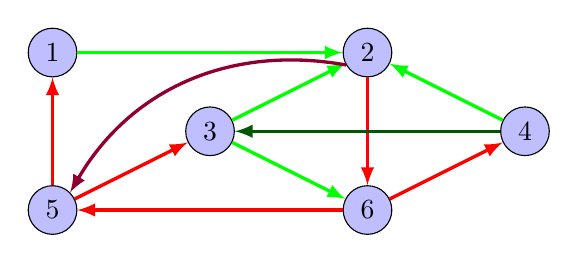
\begin{tikzpicture}
		[node/.style={circle,draw,fill=blue!25!white,minimum size=0.5cm},>=latex]
		\node[node,name=1]at(0,2){$1$};
		\node[node,name=2]at(4,2){$2$};
		\node[node,name=3]at(2,1){$3$};
		\node[node,name=4]at(6,1){$4$};
		\node[node,name=5]at(0,0){$5$};
		\node[node,name=6]at(4,0){$6$};
		\draw[->,green,very thick] (1) -- (2);
		\draw[->,green,very thick] (3) -- (2);
		\draw[->,green,very thick] (4) -- (2);
		\draw[->,green,very thick] (3) -- (6);
		\draw[->,red,very thick] (5) -- (1);
		\draw[->,red,very thick] (5) -- (3);
		\draw[->,red,very thick] (6) -- (5);
		\draw[->,red,very thick] (2) -- (6);
		\draw[->,red,very thick] (6) -- (4);
		\draw[->,green!35!black,very thick] (4) -- (3);
		\draw[->,purple!75!black,very thick] (2.210) to [bend right=35] (5.north east);
	\end{tikzpicture}}
\hfil
\subfloat[\label{fig:df2}]{
	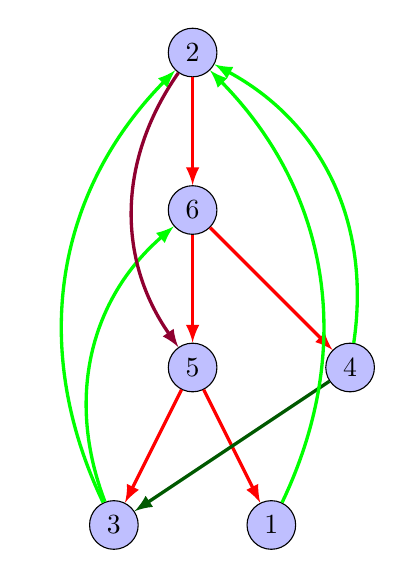
\begin{tikzpicture}
	[node/.style={circle,draw,fill=blue!25!white,minimum size=0.5cm},>=latex]
	\node[node,name=1]at(3,0){$1$};
	\node[node,name=2]at(2,6){$2$};
	\node[node,name=3]at(1,0){$3$};
	\node[node,name=4]at(4,2){$4$};
	\node[node,name=5]at(2,2){$5$};
	\node[node,name=6]at(2,4){$6$};
	\draw[->,red,very thick] (5) -- (1);
	\draw[->,red,very thick] (5) -- (3);
	\draw[->,red,very thick] (6) -- (5);
	\draw[->,red,very thick] (2) -- (6);
	\draw[->,red,very thick] (6) -- (4);
	\draw[->,green!35!black,very thick] (4) -- (3);
	\draw[->,green,very thick] (4) to [bend right = 35] (2);
	\draw[->,green,very thick] (1) to [bend right = 35] (2);
	\draw[->,green,very thick] (3) to [bend left = 35] (6);
	\draw[->,green,very thick] (3) to [bend left = 35] (2);
	\draw[->,purple!75!black,very thick] (2) to [bend right = 35] (5);
\end{tikzpicture}
}
\caption{}
\end{figure}

L'algoritmo \textsc{DFS} può essere utilizzato per classificare gli archi di un grafo $G$. In particolare, si usa il colore del vertice che si raggiunge durante la visita dell'arco $(u,v)$ per effettuare la discriminazione tra le varie tipologie:
\begin{itemize}
	\item Se $v$ è bianco allora l'arco è un \textbf{\textcolor{red}{arco d'albero}};
	\item Se $v$ è grigio allora l'arco è un \textbf{\textcolor{green}{arco di ritorno}};
	\item Se $v$ è nero allora l'arco è un \textbf{\textcolor{purple!75!black}{arco in avanti}} o un \textbf{\textcolor{green!35!black}{arco di attraversamento}}:
	\begin{itemize}
		\item se inoltre $d[u]<d[v]$ allora è un \textbf{\textcolor{purple!75!black}{arco in avanti}};
		\item se inoltre $d[v]<d[u]$ allora è un \textbf{\textcolor{green!35!black}{arco di attraversamento}}.
	\end{itemize}
\end{itemize}
È possibile quindi modificare l'algoritmo \textsc{DFS-Visit}$(G,s)$ per visualizzare la tipologia di tutti gli archi ispezionati:
\begin{lstlisting}[language=asd,caption={Print-DFS-Visit(G,s)}]
Color[s] = Gray
time = time+1
d[s] = time
for each v @$\in$@ Adj(s) do
	if Color[v] = White then
		print("(s,v) e' d'albero")
		Pred[v] = s
		DFS-Visit(G,v)
	else
		if Color[v] = Gray then
			print("(s,v) e' all'indietro")
		else if(d[s]<d[v]) then
			print("(s,v) e' in avanti")
		else
			print("(s,v) e' d'attraversamento")
time = time+1
f[s] = time
Color[s] = Black
\end{lstlisting}

\subsection{Verifica dei grafi aciclici}
Grazie alla caratterizzazione degli archi appena visti possiamo osservare che l'algoritmo \textsc{DFS} è in grado di verificare se un grafo è \textbf{ciclico} o meno. Se si osservano attentamente i grafi mostrati in Figura \ref{fig:grafo1} e \ref{fig:grafo2} notiamo infatti la presenza di vari cicli che vengono descritti dagli archi etichettati di verde chiaro, ovvero gli archi all'indietro.

Assumiamo che $G=(V,E)$ sia un grafo orientato in cui ci sia un ciclo semplice $\langle v_{1},v_{2},\ldots,v_{k} \rangle$ e sia $v_{1}$ il primo vertice scoperto dalla \textsc{BFS}. Nell'istante $d[v_{1}]$ gli altri vertici sono bianchi, quindi, per il teorema del percorso bianco esiste un percorso bianco da $v_{1}$ a $v_{2},v_{2}, \ldots, v_{i}$ per $i=\{2,3,\ldots,k\}$. Se esiste tale percorso bianco allora i vertici $v_{2},v_{3}, \ldots, v_{i}$ sono discendenti di $v_{1}$ e gli archi di tale percorso sono archi dell'albero. Una volta arrivati al vertice $v_{k}$ l'unico arco ancora da percorrere è quello che lo conduce all'antenato $v_{1}$ e tale arco risulta quindi un arco all'indietro.
\begin{center}
	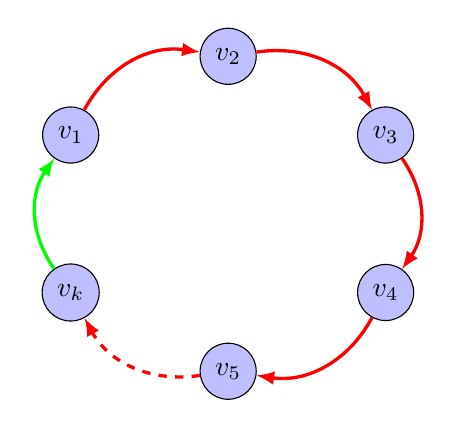
\begin{tikzpicture}
	[node/.style={circle,draw,fill=blue!25!white,minimum size=0.5cm},>=latex]
	\node[node,name=1]at(1,5){$v_{1}$};
	\node[node,name=2]at(3,6){$v_{2}$};
	\node[node,name=3]at(5,5){$v_{3}$};
	\node[node,name=4]at(5,3){$v_{4}$};
	\node[node,name=5]at(3,2){$v_{5}$};
	\node[node,name=6]at(1,3){$v_{k}$};
	\draw[->,red,very thick](1) to[bend left=35] (2);
	\draw[->,red,very thick](2) to[bend left=35] (3);
	\draw[->,red,very thick](3) to[bend left=35] (4);
	\draw[->,red,very thick](4) to[bend left=35] (5);
	\draw[->,dashed,red,very thick](5) to[bend left=35] (6);
	\draw[->,green,very thick](6) to[bend left=35] (1);
	\end{tikzpicture}
\end{center}

È possibile quindi definire un algoritmo il quale, dato un grafo orientato, restituisca \texttt{true} se aciclico e \texttt{false} altrimenti.
\begin{minipage}{.4\textwidth}
	\begin{lstlisting}[language=asd,caption={\textsc{Aciclico}(G)}]
		Init(G)
		for each v @$\in$@ V do
			if Color[v] = White then
				ret = Aciclico-Visit(G,v)
				if ret = false then
					return false
		return true
	\end{lstlisting}
\end{minipage}
\begin{minipage}{.4\textwidth}
	\begin{lstlisting}[caption={\textsc{Aciclico-Visit}(G,s)},language=asd]
		Color[s] = Gray
		for each v @$\in$@ Adj(s) do
			if Color[v] = White then
				ret = Aciclico-Visit(G,v)
				if ret = false then
					return false
			else
				if Color[v] = Gray then
					return false
		return true
	\end{lstlisting}
\end{minipage}
\newpage

\section{Ordinamento topologico in un grafo}
\subsection{Relazione d'ordine nei grafi}
\dfn{Ordinamento topologico}{
	Sia $G=(V,E)$ un grafo orientato aciclico, si definisce \textbf{ordinamento topologico} di $G$ una permutazione $\pi$ di $V$ tale che:
	\begin{equation}
		\forall (v,u) \in E, \quad \text{$v$ precede $u$ in $\pi$}
	\end{equation}
	Se due vertici $v$ e $u$ sono presenti in un ordinamento topologico allora si diranno \textit{confrontabili} e lo si indica con $v < u$.
}

\begin{example}
Si consideri il seguente grafo:
\begin{center}
	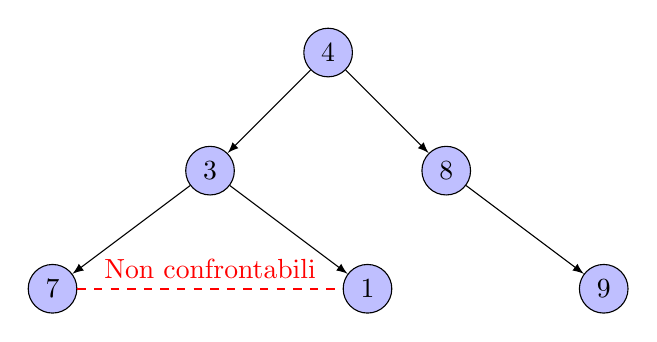
\begin{tikzpicture}
	[node/.style={circle,draw,fill=blue!25!white,minimum size=0.5cm},>=latex, level 1/.style={sibling distance=3cm},level 2/.style={sibling distance=4cm}]
\node[node]{4}
child[->]{
	node[node]{3}
	child{
		node[node,name=1]{7}
	}
	child{
		node[node,name=2]{1}
	}
}
child[->]{
	node[node]{8}
	child[missing]
	child{
		node[node]{9}
	}
};
\draw[-,dashed,red,thick](1)--node[above]{Non confrontabili}(2);
\end{tikzpicture}
\end{center}
È possibile ricavare le seguenti relazioni:
\begin{displaymath}
	\begin{array}{ll}
		4 < 3 &		4 < 8\\
		4 < 7 &		4 < 1\\
		4< 9 &		3 < 7\\
		3 < 1 &		8 < 9\\
	\end{array}
\end{displaymath}
Notare il fatto che non è possibile determinare alcuna relazione tra i vertici $7$ ed $1$ oppure $3$ ed $8$ in quanto non esiste alcun arco in $G$ che li collega. In generale, infatti, la struttura del grafo induce una relazione d'ordine \textit{parziale}.
\end{example}


\begin{osservation}
		Se nel grafo sono presenti cicli non è possibile determinare alcun ordinamento topologico. Infatti, preso ad esempio il seguente grafo:
	\begin{center}
		\begin{tikzpicture}
			[node/.style={circle,draw,fill=blue!25!white,minimum size=0.5cm},>=latex]
			\node[node,name=1]{$v_{1}$};
			\node[node,name=2,right=4cm of 1]{$v_{2}$};
			\draw[->,very thick](1.north) to[bend left=25](2.north);
			\draw[->,very thick](2.south)to[bend left=25](1.south);
		\end{tikzpicture}
	\end{center}
	non è possibile determinare quale nodo preceda l'altro all'interno di un possibile ordinamento. Lo stesso ragionamento vale anche nel caso in cui si considerano i grafi non orientati dove non è definito il concetto di precedenza. Per questo motivo, la nozione di ordinamento topologico si applica solo ai grafi orientati aciclici.
\end{osservation}


\begin{osservation}
		Dato un grafo orientato $G=(V,E)$ è possibile ricavare più di un ordinamento topologico. Nel caso in cui l'insieme $E$ sia vuoto (grafo senza archi) allora il numero di permutazioni possibili corrisponde a $|V|!$. Nel caso in cui il grafo si riduca ad una sequenza di vertici è possibile avere un unico ordinamento topologico. Si consideri ad esempio il seguente grafo:
	\begin{center}
		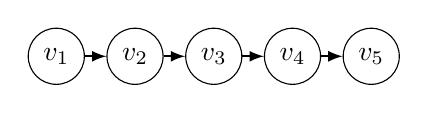
\begin{tikzpicture}
			[node/.style={circle,draw,fill=white,minimum size=0.5cm},>=latex]
			\node[node,name=1]at(0,0){$v_{1}$};
			\node[node,name=2]at(1,0){$v_{2}$};
			\node[node,name=3]at(2,0){$v_{3}$};
			\node[node,name=4]at(3,0){$v_{4}$};
			\node[node,name=5]at(4,0){$v_{5}$};
			\draw[->,thick] (1)--(2);
			\draw[->,thick] (2)--(3);
			\draw[->,thick] (3)--(4);
			\draw[->,thick] (4)--(5);
		\end{tikzpicture}
	\end{center}
	Tale grafo ammette un unico ordinamento topologico dato dalla permutazione $\pi=\langle v_{1},v_{2},v_{3},v_{4},v_{5} \rangle$. Tale ordinamento non è solo l'unico ma anche totale.
\end{osservation}

\subsection{Proprietà dei grafi aciclici}


\begin{propbox}
		Se $G=(V,E)$ è un grafo aciclico e $G'$ è un suo sottografo allora $G'$ è aciclico.
\end{propbox}

\begin{proof}
	Per ipotesi si ha $G' = (V',E') $, con:
\begin{displaymath}
\begin{array}{c}
			V' \subseteq V \\
			E' \subseteq E \cap (V' \times V')
\end{array}
\end{displaymath}
Supponiamo per assurdo che $G'$ sia un grafo ciclico e consideriamo un percorso ciclico di $G'$, sia esso $\pi$:
\begin{displaymath}
	\pi = \langle v_{1}, v_{2}, \cdots, v_{k}, v_{1}\rangle
\end{displaymath}
Chiaramente ciascun arco nel percorso $\pi$ è un arco presente in $E'$. Poiché $E'$ è un sottoinsieme di $E$, quindi ogni arco di $\pi$ appartiene ad $E$ e $\pi$ risulta quindi un percorso in $G$ che di fatto risulta ciclico, contro le nostre ipotesi.
\end{proof}

\begin{propbox}
	Se $G$ è un grafo aciclico allora esiste almeno un vertice $v \in V$ tale che $v$ ha grado entrante pari a $0$.
\end{propbox}


\begin{proof}
	Ragionando per contrapposizione supponiamo che per ogni vertice di $V$ ci sia almeno un arco entrante. Senza ledere di generalità consideriamo un vertice di $V$, tale $v_{1}$. Per l'ipotesi appena posta esiste almeno un arco che entra in $v_{1}$ ed esiste quindi un vertice $v_{2} \neq v_{1}$ dal quale si diparte tale arco. Ragionando allo stesso modo possiamo considerare un arco che parta da un vertice $v_{3}$ e arrivi in $v_{2}$ e così via fino ad arrivare all'ultimo vertice $v_{n} \in V$.  Poiché il grado entrante di $v_{n}$ è maggiore di $1$ ciò significa che esiste almeno un arco che parte da uno dei vertici $\{v_{1},\ldots, v_{n-1}\}$ (non potrebbe essere altrimenti) e arriva in $v_{n}$. Ciò, però, dimostra l'esistenza di un percorso ciclico nel grafo $G$, il quale per ipotesi era stato definito aciclico. Mostrato l'assurdo si dimostra l'enunciato.
\begin{center}
	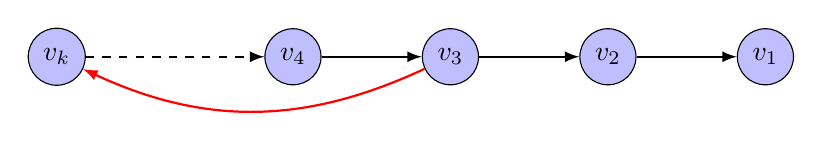
\begin{tikzpicture}
		[node/.style={circle,draw,fill=blue!25!white,minimum size=0.5cm},>=latex]
		\node[node,name=1]at(0,0){$v_{1}$};
		\node[node,name=2]at(-2,0){$v_{2}$};
		\node[node,name=3]at(-4,0){$v_{3}$};
		\node[node,name=4]at(-6,0){$v_{4}$};
		\node[node,name=5]at(-9,0){$v_{k}$};
		\draw[->,thick] (2)--(1);
		\draw[->,thick] (3)--(2);
		\draw[->,thick] (4)--(3);
		\draw[->,thick,dashed] (5)--(4);
		\draw[->,red,thick](3) to [bend left=25] (5);
	\end{tikzpicture}
\end{center}
\end{proof}



\begin{propbox}
		Dato un grafo aciclico $G=(V,E)$, se $G$ è aciclico allora esiste almeno un ordinamento topologico di $G$.
\end{propbox}


\begin{proof}
	Dato che $G$ è aciclico esiste almeno un vertice $v_{1} \in V$ con grado entrante pari a zero. Chiaramente un vertice del genere deve essere posto all'inizio di qualsiasi ordinamento topologico $\pi$ in quanto non esiste alcun vertice che lo preceda. Escluso tale vertice possiamo quindi considerare il sottografo: $$G_{1}=(V\setminus\{v_{1}\},E \setminus \{(v_{1},u)\in E \; | \; u \in V\})$$ ottenuto rimuovendo $v_{1}$ da $V$ e ciascun arco che collegava $v_{1}$.
\begin{center}
	\begin{tikzpicture}
		[node/.style={circle,draw,fill=blue!25!white,minimum size=0.5cm},>=latex]
		\node[node,name=1]at(0,0){};
		\node[node,name=2]at(-3,-0.5){};
		\node[node,name=3]at(-5,-1){};
		\node[node,name=4]at(-6,0){};
		\node[node,name=5]at(-9,-1){};
		\draw[->,thick] (2)--(1);
		\draw[->,thick] (3)--(2);
		\draw[->,thick] (4)--(3);
		\draw[->,thick](4)--(2);
		\draw[->,thick,dashed] (5)--(4);
		\draw[->,thick,dashed](5)--(3);
		\node[thick,draw=blue,name=r1,shape=rectangle,fit={(1)(2)(3)(4)}]{};
		\node[below=0.2cm of r1,font=\color{blue}\bfseries]{$G_{1}$};
	\end{tikzpicture}
\end{center}
Chiaramente, essendo $G_{1}$ un sottografo di un grafo aciclico, anche $G_{1}$ risulta aciclico e quindi esisterà un vertice $v_{2}$ con grado entrante pari a zero. Tale vertice può essere quindi inserito a destra del vertice $v_{1}$ all'interno dell'ordinamento topologico $\pi$. È possibile iterare questo procedimento fino a quando non si raggiunge il sottografo vuoto, ottenendo così l'ordinamento topologico:
\[\pi = (v_{1},v_{2},\ldots, v_{k})\]
\end{proof}


\begin{proof}
	Chiaramente, l'ordinamento topologico così ottenuto dipende dalla scelta del vertice $v_{i}$ con grado entrante pari a zero il quale può essere più di uno. All'interno di uno stesso grafo, infatti, l'ordine dei vertici con grado entrante pari a zero all'interno di una permutazione è indifferente e possono quindi essere messi uno dopo o prima dell'altro.
\end{proof}

\begin{example}
	Consideriamo il seguente grafo:
	\begin{center}
		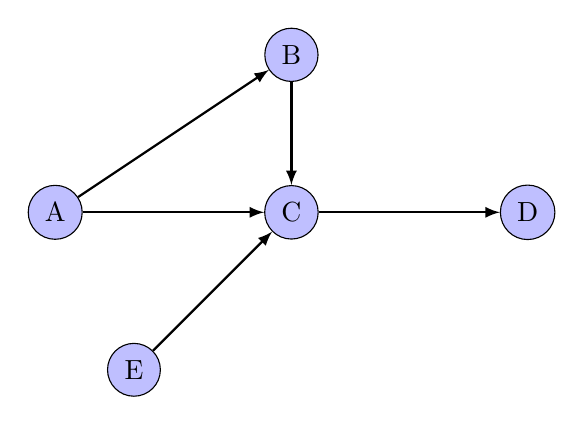
\begin{tikzpicture}
			[node/.style={circle,draw,fill=blue!25!white,minimum size=0.5cm},>=latex]
			\node[node,name=a]at(0,0){A};
			\node[node,name=b]at(3,2){B};
			\node[node,name=c]at(3,0){C};
			\node[node,name=d]at(1,-2){E};
			\node[node,name=e]at(6,0){D};
			\draw[->,thick](a) --(b);
			\draw[->,thick](b) --(c);
			\draw[->,thick](a) --(c);
			\draw[->,thick](c) --(e);
			\draw[->,thick](d) --(c);
		\end{tikzpicture}
	\end{center}
In questo caso esistono due vertici con grafo entrante pari a zero: il vertice A  ed il vertice E. Possiamo quindi scegliere uno qualsiasi tra i due come primo elemento della permutazione $\pi$. Scelto il vertice A si ottiene:
\begin{center}
	\begin{tikzpicture}
		[node/.style={circle,draw,fill=blue!25!white,minimum size=0.5cm},>=latex]
		\node[node,name=a,opacity=0.2]at(0,0){A};
		\node[node,name=b]at(3,2){B};
		\node[node,name=c]at(3,0){C};
		\node[node,name=d]at(1,-2){E};
		\node[node,name=e]at(6,0){D};
		\node[shape=rectangle,name=g1,draw=red,fit={(b)(c)(d)(e)}]{};
		\node[below=0.5cm of g1,font=\color{red}\bfseries]{$G_{1}$};
		\node[right=0.5cm of g1,font=\bfseries]{$\pi=(A)$};
		\draw[->,thick,opacity=0.2](a) --(b);
		\draw[->,thick](b) --(c);
		\draw[->,thick,opacity=0.2](a) --(c);
		\draw[->,thick](c) --(e);
		\draw[->,thick](d) --(c);
	\end{tikzpicture}
\end{center}
Il sottografo $G_{1}$ così ottenuto ha ancora due vertici con grado entrante pari a zero: B ed E. Scelto quindi il vertice E si ottiene il nuovo sottografo $G_{2}$:
\begin{center}
	\begin{tikzpicture}
		[node/.style={circle,draw,fill=blue!25!white,minimum size=0.5cm},>=latex]
		\node[node,name=a,opacity=0.2]at(0,0){A};
		\node[node,name=b]at(3,2){B};
		\node[node,name=c]at(3,0){C};
		\node[node,name=d,opacity=0.2]at(1,-2){E};
		\node[node,name=e]at(6,0){D};
		\node[shape=rectangle,name=g1,draw=red,fit={(b)(c)(e)}]{};
		\node[below=0.5cm of g1,font=\color{red}\bfseries]{$G_{2}$};
		\node[right=0.5cm of g1,font=\bfseries]{$\pi=(A,E)$};
		\draw[->,thick,opacity=0.2](a) --(b);
		\draw[->,thick](b) --(c);
		\draw[->,thick,opacity=0.2](a) --(c);
		\draw[->,thick](c) --(e);
		\draw[->,thick,opacity=0.2](d) --(c);
	\end{tikzpicture}
\end{center}
Il grafo $G_{2}$, così come il resto dei suoi sottografi ottenuti iterando il procedimento, hanno un unico vertice con grado entrante pari a zero, è quindi univoca la sequenza dei vertici estratti. Si ottiene così l'ordinamento topologico: $$\pi=(A,E,B,C,D)$$
\end{example}

\subsection{Algoritmo del grado entrante}
Per trasformare la procedura appena studiata in un algoritmo che determini un ordinamento topologico bisogna capire come calcolare il \textit{grado entrante} di ogni vertice per poter selezionare i vertici con grado entrante nullo. Le liste di adiacenza non sono adatte a fornire tale informazione in quanto esprimono (mediante la loro dimensione) soltanto il grado uscente di ogni vertice.

Chiaramente, il grado entrante di un vertice può essere ottenuto dalla dimensione della sua \textbf{lista di incidenza}, ovvero una lista che descrive tutti i vertici dai quali si dipartono degli archi orientati verso il vertice selezionato\footnote{Qualora il grafo fosse stato implementato mediante matrici di adiacenza sarebbe stato sufficiente calcolare la sua trasposta}. La generazione di tali liste, però, risulta essere un'operazione costosa in quanto richiede di scorrere l'intero insieme degli archi. Per questo motivo, si preferisce utilizzare un algoritmo che calcoli il grado entrante di ogni vertice in modo più efficiente.
% Explain how the SortingTopology algorithm works, in particular how the indegrees of each vertex are calculated.
L'Algoritmo \ref{lst:GradoEntrante} imposta innanzitutto il grado entrante di ogni vertice a $0$ e poi, per ogni vertice $v \in V$, incrementa il grado entrante di tutti i vertici adiacenti ad $v$. Chiaramente, l'algoritmo risulta essere lineare sulla dimensione del grafo.

Calcolato il grado entrante di ciascun vertice è possibile implementare l'algoritmo \ref{lst:OrdTop} che, partendo dai vertici con grado entrante pari a zero, li inserisce in una coda $Q$ e li estrae uno alla volta. Per ogni vertice estratto $v$ si itera sui suoi adiacenti $u$ e si decrementa il loro grado entrante. Se il grado entrante di $u$ diventa pari a zero allora viene inserito nella coda $Q$. L'algoritmo termina quando la coda $Q$ risulta vuota.

\begin{lstlisting}[caption={\textsc{OrdinamentoTopologico}(G)},language=asd,label=lst:OrdTop]
  Q = NIL
  // Funzione che associa ad ogni vertice il proprio grado entrante
  Ge = GradoEntrante(G)
  for each v @$\in$@ V do
    // Accodo i vertici con grado zero
    if Ge[v]=0 then
      Q = Enqueue(Q,v)
  while (Q @$\neq$@ NIL) do
    v = Head(Q)
    print(v)
    // Aggiorno il grado entrante degli adiacenti
    for each u @$\in$@ Adj[v] do
      Ge[u] = Ge[u]-1
      if Ge[u]=0 then
        Q = Enqueue(Q,u)
      Q= Dequeue(Q)
\end{lstlisting}
\begin{lstlisting}[language=asd,caption={\textsc{GradoEntrante}(G)},label=lst:GradoEntrante]
for each v @$\in$@ V do
  Ge[v] =0
for each v @$\in$@ V do
  for each u @$\in$@ Adj[v] do
    Ge[u]=Ge[u]+1
return Ge
\end{lstlisting}

Chiaramente, l'algoritmo \ref{lst:OrdTop} risulta lineare sulla dimensione del grafo. Infatti:
\begin{eqnarray*}
	T_{OrdinamentoTopologico} &=& T_{GradoEntrante} + |V| + (|V|+|E|)\\
	&=& (|V|+|E|) + |V| + (|V|+|E|) \\
	&=& 3 \cdot |V| + 2 \cdot |E| \\
	&\simeq& |V| + |E|
\end{eqnarray*}

\subsection{Calcolo dell'ordinamento topologico mediante DFS}
È possibile calcolare l'ordinamento topologico di un grafo mediante l'algoritmo \textsc{DFS} in modo molto semplice. Infatti, l'ordinamento topologico di un grafo $G$ è semplicemente l'ordinamento inverso dei tempi di fine visita dei vertici di $G$. Infatti, se $G$ è aciclico allora non esistono archi all'indietro e quindi non esistono archi che collegano vertici con tempi di fine visita diversi. Inoltre, se $G$ è aciclico allora esiste almeno un vertice con grado entrante pari a zero e quindi tale vertice sarà il primo ad essere visitato dall'algoritmo \textsc{DFS}. Il vertice successivo da visitare sarà il vertice adiacente al primo e così via. Sfruttando questa osservazione è possibile inserire i vertici in uno stack man mano che questi vengono visitati. Una volta terminata la visita, basterà estrarre i vertici dallo stack per ottenere l'ordinamento topologico. L'algoritmo \ref{lst:OrdTopDFS} mostra come implementare tale procedura.

Il tempo di esecuzione di tale algoritmo è pari a quello dell'algoritmo \textsc{DFS}. Infatti, l'unico costo aggiuntivo è quello di inserire i vertici nello stack, operazione che richiede tempo costante. L'ordinamento topologico viene quindi calcolato in tempo lineare sulla dimensione del grafo.
	\begin{lstlisting}[language=asd,caption={\textsc{OrdinamentoTopologico-DFS}(G)},label=lst:OrdTopDFS]
	tempo = 0
	Init(G)
	S = NIL
	for each v @$\in$@ V do
		if Color[v] = White then
			S = OrdinamentoTopologico-DFS-Visit(G,v,S)
	return S
\end{lstlisting}



	\begin{lstlisting}[language=asd,caption={\textsc{OrdinamentoTopologico-DFS-Visit}(G,v,S)},label=lst:OrdTopDFSVisit]
	Color[v] = Gray
	time = time+1
	d[v] = time
	for each u @$\in$@ Adj[v] do
		if Color[u] = White then
			S = OrdinamentoTopologico-DFS-Visit(G,u,S)
	time = time+1
	f[v] = time
	Color[v] = Black
	S = Push(S,v)
	return S
\end{lstlisting}


\section{Calcolo delle componenti fortemente connesse}

Il concetto di \textbf{componente fortemente connessa} è strettamente legato al concetto di grafo fortemente connesso.

\dfn{Raggiungibilità e connessione}{
	Un grafo non orientato è \textbf{connesso} se ogni coppia di vertici è collegata attraverso un cammino.  Le \textbf{componenti connesse} di un grafo è un insieme di coppie di vertici che soddisfano la condizione di raggiungibilità. Un grafo orientato è \textbf{fortemente connesso} se due vertici qualsiasi sono raggiungibili l'uno con l'altro. Se $G$ è un grafo orientato non fortemente connesso, ed il grafo non orientato sottostante è connesso, allora si dice che $G$ è \textbf{debolmente connesso}.
}

\begin{example}
	Ad esempio, il grafo non orientato $G=(V,E)$ mostrato in Figura \ref{fig:grafoconnesso1} è un grafo connesso, infatti ogni vertice è raggiungibile da qualsiasi altro vertice. Al contrario, il grafo non orientato mostrato in Figura \ref{fig:grafoconnesso2} non è un grafo connesso in quanto non tutti i vertici sono reciprocamente raggiungibili, in questo caso il grafo è detto \textbf{sconnesso}.
	\begin{center}
		\begin{minipage}{.45\textwidth}
			\centering
			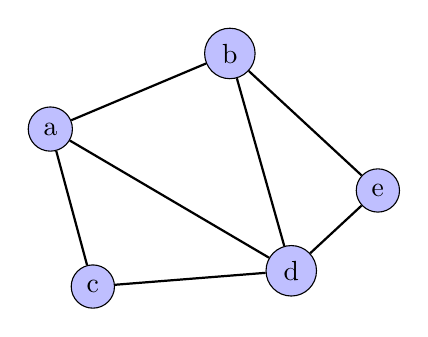
\begin{tikzpicture}
			[node/.style={circle,draw,fill=blue!25!white,minimum size=0.5cm},>=latex]
			\node[node,name=1] at (0.84,4) {a};
			\node[node,name=2]at (3.12,4.96) {b};
			\node[node,name=3]at (1.38,2){c};
			\node[node,name=4]at(3.9,2.2){d};
			\node[node,name=5]at(5,3.22){e};
			\draw[-,thick](1)--(2);
			\draw[-,thick](1)--(3);
			\draw[-,thick](1)--(4);
			\draw[-,thick](2)--(4);
			\draw[-,thick](2)--(5);
			\draw[-,thick](4)--(5);
			\draw[-,thick](3)--(4);
		\end{tikzpicture}
	\captionof{figure}{}\label{fig:grafoconnesso1}
		\end{minipage}
	\begin{minipage}{.45\textwidth}
		\centering
		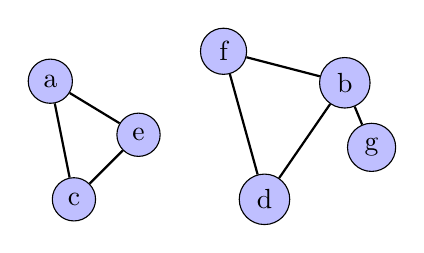
\begin{tikzpicture}
			[node/.style={circle,draw,fill=blue!25!white,minimum size=0.5cm},>=latex]
			\node[node,name=a] at (0.84,4) {a};
			\node[node,name=b]at (4.58,3.98) {b};
			\node[node,name=c]at (1.14,2.5){c};
			\node[node,name=d]at(3.56,2.5){d};
			\node[node,name=e]at(1.96,3.32){e};
			\node[node,name=f]at(3.04,4.38){f};
			\node[node,name=g]at(4.92,3.16){g};
			\draw[-,thick](a)--(e);
			\draw[-,thick](e)--(c);
			\draw[-,thick](c)--(a);
			\draw[-,thick](f)--(b);
			\draw[-,thick](g)--(b);
			\draw[-,thick](d)--(b);
			\draw[-,thick](d)--(f);
		\end{tikzpicture}
	\captionof{figure}{}\label{fig:grafoconnesso2}
	\end{minipage}
	\end{center}
\end{example}

\dfn{Componente fortemente connessa}{
	Una \textbf{componente fortemente connessa} di un grafo orientato $G=(V,E)$ è un insieme massimale di vertici $C \subseteq V$ tale che per ogni coppia di vertici $u,v \in C$ si ha $	u  \leadsto v $ e anche $ v \leadsto u$; ovvero i vertici $u$ e $v$ sono raggiungibili l'uno dall'altro.
}


\begin{osservation}
	Se in un grafo orientato esistono vertici mutualmente raggiungibili vuol dire che il grafo è ciclico.
\end{osservation}


\begin{example}
Si consideri il grafo $G$ in Figura \ref{fig:example_strongly_connected_graph}. Tale grafo contiene quattro componenti fortemente connesse: $C_{1},C_{2},C_{3}$ e $C_{4}$.
\begin{center}
		\begin{tikzpicture}
		[node/.style={circle,draw,fill=blue!25!white,minimum size=0.5cm},>=latex]
		\node[node,name=1]at (0,0){};
		\node[node,name=2]at(1.5,0){};
		\node[node,name=3]at(3.25,0){};
		\node[node,name=4]at(5,0){};
		\node[node,name=5]at(6,-1){};
		\node[node,name=6]at(7,0){};
		\node[node,name=7]at(2,-1.5){};
		\node[node,name=8]at(3,-2.5){};
		\node[node,name=9]at(1,-2.5){};
		\node[node,name=10]at(2,-3.5){};
		\draw[->,thick](1) to [bend left=45](2);
		\draw[->,thick](2) to [bend left=45](1);
		\draw[->,thick](2) --(3);
		\draw[->,thick](3) --(4);
		\draw[->,thick](4) --(5);
		\draw[->,thick](5) --(6);
		\draw[->,thick](6) --(4);
		\draw[->,thick](7) --(8);
		\draw[->,thick](8) --(9);
		\draw[->,thick](9) --(10);
		\draw[->,thick](10) --(7);
		\draw[->,thick](10) --(8);
		\draw[->,thick](7) --(9);
		\draw[->,thick](7) --(3);
		\draw[->,thick](1) to [bend right=30](9);
		\node[draw=green,dashed,shape=ellipse,fit={(1)(2)},name=c1]{};
		\node[anchor=south,font=\color{green}\bfseries]at(c1.north){$C_{1}$};
		\node[draw=red,dashed,shape=ellipse,fit={(3)},name=c3]{};
		\node[anchor=south,font=\color{red}\bfseries]at(c3.north){$C_{3}$};
		\node[draw=blue,dashed,shape=ellipse,fit={(4)(5)(6)},name=c4]{};
		\node[anchor=south,font=\color{blue}\bfseries]at(c4.north){$C_{4}$};
		\node[draw=orange,dashed,shape=ellipse,fit={(7)(8)(9)(10)},name=c2]{};
		\node[anchor=north,font=\color{orange}\bfseries]at(c2.south){$C_{2}$};
	\end{tikzpicture}
\captionof{figure}{Un grafo orientato $G$}\label{fig:example_strongly_connected_graph}
\end{center}
\end{example}


La relazione di reciproca raggiungibilità $RR$ in un grafo $G=(V,E)$ è una relazione di equivalenza. Infatti, essa è:
\begin{itemize}
	\item \textbf{riflessiva}: ogni vertice è raggiungibile da se stesso;
	\item \textbf{simmetrica}: se $u$ è raggiungibile da $v$ allora $v$ è raggiungibile da $u$;
	\item \textbf{transitiva}: se $u$ è raggiungibile da $v$ e $v$ è raggiungibile da $w$ allora $u$ è raggiungibile da $w$.
\end{itemize}

Per questo motivo è possibile definire le \textbf{classi di equivalenza} indotte dalla relazione di mutua raggiungibilità. Ogni classe di equivalenza è una componente fortemente connessa. Infatti, se due vertici sono mutualmente raggiungibili allora questi apparterranno alla stessa componente fortemente connessa.

\dfn{Grafo delle componenti}{
L'insieme quoziente della relazione $RR$, ovvero l'insieme di tutti gli insiemi di vertici mutualmente raggiungibili, è detto \textbf{insieme delle componenti fortemente connesse} di $G$ ed è rappresentato mediante il \textbf{grafo delle componenti} $G_{CFC}$ il quale è equivalente a $G$:

\begin{equation}
	G_{CFC}=(V_{CFC},E_{CFC})
\end{equation}

dove $V_{CFC}$ contiene un nodo per ogni componente fortemente connessa di $G$ e
\[E_{CFC} = \{(u,v) \; | \; u,v \in V_{CFC}, \exists \text{ un arco in $E$ da un vertice $u$  o un vertice $v$}\}\]
}

\begin{propbox}
	Sia $G=(V,E)$ un grafo, allora $u \in V $ è raggiungibile dal vertice $v \in V$ se e soltanto se esiste un percorso da un qualsiasi vertice della componente fortemente connessa di $u$ ad un qualsiasi vertice della componente fortemente connessa di $v$.
\end{propbox}

Data questa proprietà possiamo osservare che il \textbf{problema della raggiungibilità} tra due vertici può essere studiato decomponendolo mediante l'analisi del grafo delle componenti. Bisogna trovare quindi il modo di calcolare le componenti fortemente connesse presenti in un grafo.

\begin{example}
	Il grafo delle componenti del grafo mostrato in Figura \ref{fig:example_strongly_connected_graph} risulta:
	\begin{center}
		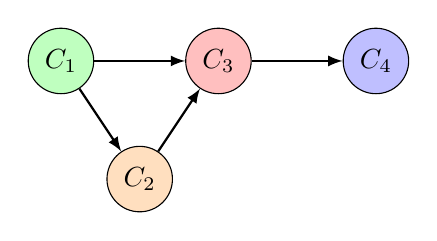
\begin{tikzpicture}
			[node/.style={circle,draw,minimum size=0.5cm},>=latex]
			\node[node,name=1,fill=green!25!white]at(0,0){$C_{1}$};
			\node[node,name=2,fill=red!25!white]at(2,0){$C_{3}$};
			\node[node,name=3,fill=blue!25!white]at(4,0){$C_{4}$};
			\node[node,name=4,fill=orange!25!white]at(1,-1.5){$C_{2}$};
			\draw[->,thick](1)--(2);
			\draw[->,thick](2)--(3);
			\draw[->,thick](4)--(2);
			\draw[->,thick](1)--(4);
		\end{tikzpicture}
	\end{center}
il che rappresenta una forma molto più compatta, che preserva ancora le informazioni relative alla raggiungibilità dei vertici, del grafo $G$.
\end{example}


\warning{Attenzione}{
	Il grafo delle componenti è \textbf{sempre aciclico}. Infatti, se esistesse un ciclo tra due componenti fortemente connesse queste apparterrebbero alla stessa classe di equivalenza del grafo connesso.
}


Nei grafi orientati, la relazione di equivalenza di raggiungibilità e reciproca raggiungibilità non si equivalgono. Si osservino infatti i seguenti grafi, nella loro versione orientata e non:
	\begin{center}
		\begin{minipage}{.45\textwidth}
			\centering
			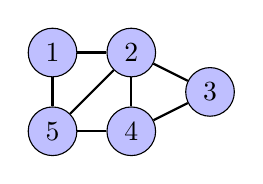
\begin{tikzpicture}
				[node/.style={circle,draw,fill=blue!25!white,minimum size=0.5cm}]
				\node[node,name=1] at (0,1) {1};
				\node[node,name=2] at (1,1) {2};
				\node[node,name=3] at (2,0.5) {3};
				\node[node,name=5] at (0,0) {5};
				\node[node,name=4] at (1,0) {4};
				\draw[thick] (1)--(2);
				\draw[thick] (1)--(5);
				\draw[thick] (2)--(3);
				\draw[thick] (2)--(4);
				\draw[thick] (2)--(5);
				\draw[thick] (3)--(4);
				\draw[thick] (5)--(4);
			\end{tikzpicture}
			\captionof{figure}{{Grafo non orientato $A$}}
		\end{minipage}
		\hfil
		\begin{minipage}{.45\textwidth}
			\centering
			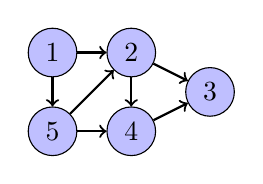
\begin{tikzpicture}
				[node/.style={circle,draw,fill=blue!25!white,minimum size=0.5cm}]
				\node[node,name=1] at (0,1) {1};
				\node[node,name=2] at (1,1) {2};
				\node[node,name=3] at (2,0.5) {3};
				\node[node,name=5] at (0,0) {5};
				\node[node,name=4] at (1,0) {4};
				\draw[thick,->] (1)--(2);
				\draw[thick,->] (1)--(5);
				\draw[thick,->] (2)--(3);
				\draw[thick,->] (2)--(4);
				\draw[thick,->] (5)--(2);
				\draw[thick,->] (4)--(3);
				\draw[thick,->] (5)--(4);
			\end{tikzpicture}
			\captionof{figure}{{Grafo orientato $B$ }}
		\end{minipage}
	\end{center}
	In un grafo non orientato ogni coppia di vertici collegati da un arco è mutualmente raggiungibile non essendo determinato alcuna orientazione e si ha $R=RR$. Al contrario, se si osserva il grafo $B$ si può osservare che i soli ed unici vertici mutualmente raggiungibili sono i singoli vertici. Cioè:
	\begin{displaymath}
		\begin{array}{l}
			R = \{(1,2),(1,5),(5,2),(2,4),(2,3),(4,3),(1,1),(2,2),(3,3),(4,4),(5,5),(5,3),(1,4),(1,3)\}\\
			RR=\{(1,1),(2,2),(3,3),(4,4),(5,5)\}
		\end{array}
	\end{displaymath}
	e vale $RR \subseteq R$. Nei grafi non orientati è sufficiente quindi verificare la raggiungibilità tra due vertici per sapere se appartengono alla stessa componente fortemente connessa.


\begin{osservation}
	Poiché la relazione di reciproca raggiungibilità determina una partizione nell'insieme dei vertici $V$ di un grafo $G$, è possibile considerare, per ogni vertice $v \in V$, il sottografo $CFC(v)$ (che corrisponde ad una classe di equivalenza), ovvero la componente fortemente connessa che contiene $v$ tra i suoi vertici (un vertice del grafo delle componenti). Chiaramente vale $CFC(v) = (V_{v},E_{v})$ dove:
\begin{displaymath}
	V_{v} = \{u \in V \; | \; \text{$u$ è reciprocamente raggiungibile con $v$}\}
\end{displaymath}
ed:
\begin{displaymath}
	E_{v}= E \cap (V_{u} \times V_{u})
\end{displaymath}
Per costruire il grafo delle componenti quindi è sufficiente trovare l'insieme $V_{v}$ (il calcolo dell'insieme $E_{v}$ è banale una volta determinato $V_{v}$) per ogni vertice del grafo $G$. Ogni componente fortemente connessa rappresenta infatti un \textbf{sottografo indotto} dalla scelta dei suoi vertici.
\end{osservation}

\subsection{Calcolo delle componenti connesse in un grafo non orientato}
Dato un grafo non orientato $G$, è possibile pensare di applicare una visita in profondità (Algoritmo \ref{lst:dfs_graph}) per risolvere il problema della raggiungibilità (e per l'osservazione precedente anche il problema della mutua raggiungibilità). Tipicamente, infatti, la DFS costruisce su $G$ una foresta, chiamata Foresta Depth First (FDF) o anche sottografo dei predecessori, costituita da alberi DF (Depth First). 

Chiaramente, tutti i vertici che appartengono ad uno stesso albero DF formano una componente connessa del grafo $G$. Possiamo quindi pensare di mappare ciascun vertice con il rispettivo albero DF di appartenenza (numerati da 1 a $k$), ottenendo così la corrispondenza che associa a ciascun vertice il ``numero'' dell'albero DF di appartenenza:
\begin{displaymath}
	CC : V \longrightarrow \mathbb{N}
\end{displaymath}
e ricavare in questo modo, per ogni $v \in V$ l'insieme $V_{v}$ ricercato.
\begin{displaymath}
	V_{v} = \{u \in V \; | \; CC[u] = CC[v] \}
\end{displaymath}

Sarà quindi sufficiente modificare l'algoritmo \textsc{DFS-Visit} in modo tale che, per ogni vertice scoperto lungo l'esplorazione del grafo, gli si associ il numero dell'albero DF che si sta attualmente costruendo.

Notiamo che la complessità temporale del meccanismo appena descritto sarà dato dal tempo della DFS che è lineare sul grafo $G$ più il tempo necessario a costruire l'insieme $V_{v}$ ovvero $k \cdot |V|$ al quale si aggiunge un costo $k \cdot |E|$ per la costruzione dei sottografi:
\begin{displaymath}
	T_{DFS_{CC}} = |V|+|E| + \bigl((k \cdot |V|) + (k\cdot|E|)\bigr)
\end{displaymath}
dove $k$ rappresenta il numero totale di componenti connesse ottenute e vale:
\begin{displaymath}
	1 \leq k \leq |V|
\end{displaymath}

\subsection{Proprietà delle componenti fortemente connesse}
\begin{teorbox}
	Se due vertici compaiono nella stessa componente fortemente connessa, allora nessun percorso tra i due vertici esce da quella componente.
\end{teorbox}

\begin{proof}
	Siano $u$ e $v$ due vertici appartenenti alla stessa componente fortemente connessa. Allora esistono percorsi sia da $v$ a $u$ che da $u$ a $v$. Sia $w$ un vertice lungo qualche percorso $	u \leadsto w \leadsto v$. Poiché c'è un percorso $v \leadsto u$, $u$ è raggiungibile da $w$ tramite $w \leadsto v \leadsto u$. Quindi $w$ e $u$ sono nella stessa componente fortemente connessa. Dall'arbitrarietà di $w$ segue l'enunciato.
\end{proof}

\begin{teorbox}
		In ogni visita DFS, tutti i vertici nella stessa componente fortemente connessa compaiono nello stesso albero depth first.
\end{teorbox}

\begin{proof}
	Sia $r$ il primo vertice di una componente fortemente connessa, visitato da \textsc{DFS} (Algoritmo \ref{lst:dfs_graph}). Poiché esso è il primo vertice ad essere scoperto allora, per il Teorema del percorso bianco (vedi \ref{sez:prop_dfs}), tutti gli altri vertici nella componente fortemente connessa devono essere ancora bianchi.

Chiaramente, per definizione di componente fortemente connessa, esiste un percorso da $r$ a tutti gli altri vertici della componente fortemente connessa. Infatti questi percorsi non escono mai dalla componente fortemente connessa di $r$ per il teorema precedente e i vertici di tutti i percorsi nella componente fortemente connessa sono bianchi. Quindi, per il teorema del percorso bianco, ogni vertice nella componente fortemente connessa sarà un discendente di $r$ nell'albero depth first.
\end{proof}

\subsection{Calcolo delle componenti fortemente connesse in un grafo orientato}
Grazie alle proprietà della visita in profondità, il calcolo delle componenti connesse risulta immediato nei grafi non orientati in quanto è stato sufficiente associare ad ogni vertice il numero dell'albero DF di appartenenza ed in base a tale numero costruire i vari sottografi $CFC(v)$.

Stessa cosa non si può dire per i grafi orientati in quanto la visita in profondità da sola non è in grado di fornire le informazioni necessarie per calcolare le componenti fortemente connesse. Infatti, il sottografo dei predecessori descrive soltanto quali vertici possono essere raggiunti dal vertice che li scopre ma non il viceversa.

Dal Teorema 2, però, osserviamo che una componente connessa non può essere divisa in due alberi DF. Quindi tutti e soli i vertici appartenenti alla componente fortemente connessa della radice si troveranno sempre e solo in unico albero depth first. Chiaramente, in un singolo albero depth first è possibile avere più componenti fortemente connesse. Per identificare una componente fortemente connessa all'interno di un albero depth first è necessario sapere quali vertici dell'albero possono raggiungere la radice $r$ dell'albero DF $T_{r}$ che li ha scoperti:
\begin{displaymath}
	CFC(r) = \{ v \in T_{r} \; | \; v \leadsto r \}
\end{displaymath}
Una volta identificata la componente fortemente connessa della radice basterà separare i vertici così ottenuti dal resto dell'albero $T_{r}$ e considerare il sottoalbero $T_{r'}$ che si ottiene rimuovendo i vertici della componente fortemente connessa e ripetere il ragionamento con la nuova radice così ottenuta.

\begin{example}
Si consideri il seguente grafo orientato mostrato in Figura \ref{fig:grafo_orientato_cfc}. Eseguendo una visita in profondità si ottengono gli alberi DF mostrati in Figura \ref{fig:grafo_orientato_cfc1} e \ref{fig:grafo_orientato_cfc2}.
\begin{center}
	\begin{minipage}{.33\textwidth}
		\centering
			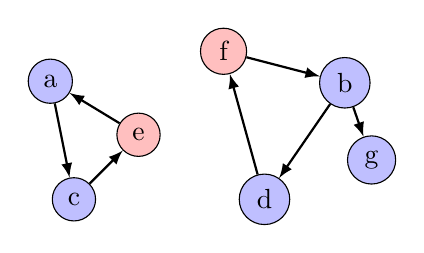
\begin{tikzpicture}
			[node/.style={circle,draw,minimum size=0.5cm,fill=blue!25!white},>=latex]
			\node[node,name=a] at (0.84,4) {a};
			\node[node,name=b]at (4.58,3.98) {b};
			\node[node,name=c]at (1.14,2.5){c};
			\node[node,name=d]at(3.56,2.5){d};
			\node[node,name=e,fill=red!25!white]at(1.96,3.32){e};
			\node[node,name=f,fill=red!25!white]at(3.04,4.38){f};
			\node[node,name=g]at(4.92,3.00){g};
			\draw[->,thick](e)--(a);
			\draw[->,thick](c)--(e);
			\draw[->,thick](a)--(c);
			\draw[->,thick](f)--(b);
			\draw[->,thick](b)--(g);
			\draw[->,thick](b)--(d);
			\draw[->,thick](d)--(f);
		\end{tikzpicture}
		\captionof{figure}{}\label{fig:grafo_orientato_cfc}
	\end{minipage}
\hfil
	\begin{minipage}{.3\textwidth}
	\centering
		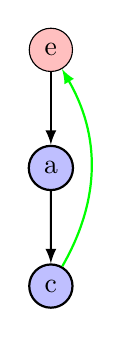
\begin{tikzpicture}
			[node/.style={circle,draw,minimum size=0.5cm,fill=blue!25!white},>=latex]
			\node[node,name=e,fill=red!25!white]{e}
			child[->,thick]{
				node[node,name=a]{a}
				child[->,thick]{
					node[node,name=c]{c}
				}
			};
			\draw[->,green,thick](c)to [bend right = 30] (e);
		\end{tikzpicture}
	\captionof{figure}{}\label{fig:grafo_orientato_cfc1}
	\end{minipage}
	\hfil
	\begin{minipage}{.3\textwidth}
	\centering
		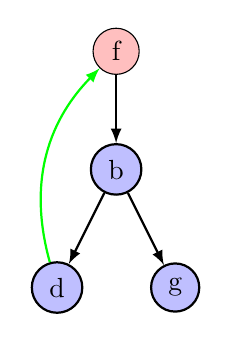
\begin{tikzpicture}
			[node/.style={circle,draw,minimum size=0.5cm,fill=blue!25!white},>=latex]
			\node[node,name=f,fill=red!25!white]{f}
			child[->,thick]{
				node[node,name=b]{b}
				child[thick,->]{
					node[node,name=d]{d}
				}
				child[->,thick]{
					node[node,name=g]{g}
				}
			};
			\draw[->,green,thick](d)to [bend left = 30] (f);
		\end{tikzpicture}
	\captionof{figure}{}\label{fig:grafo_orientato_cfc2}
	\end{minipage}
\end{center}
	Nel primo albero si osserva che tutti i vertici possono raggiungere la radice $e$ e vale quindi $CFC(e)=\{a,e,c\}$. Nel secondo albero, invece, solo i vertici $b$ e $d$ sono in grado di raggiungere la radice $f$ e vale quindi $CFC(f)=\{b,d,f\}$ mentre il vertice $g$ rappresenta la seconda CFC presente nell'albero, $CFC(g)=\{g\}$.
\end{example}

Per calcolare quali vertici sono in grado di raggiungere la radice $r$ di un albero DF in maniera efficiente è possibile utilizzare il concetto di \textbf{grafo trasposto}.

\dfn{Grafo trasposto}{
Si consideri un grafo orientato $G=(V,E)$, si definisce \textbf{grafo trasposto} il grafo il grafo $G^{T}=(V,E^{T})$ ottenuto invertendo l'orientamento degli archi del grafo $G=(V,E)$.
\begin{displaymath}
	E^{T} = \{(u,v) \; : \; (v,u) \in E \}
\end{displaymath}
}

\begin{example}
	Considerato il grafo $G$ visto nella Figura \ref{fig:grafo_orientato_cfc}, il grafo trasposto $G^{T}$ risulta:
\begin{center}
	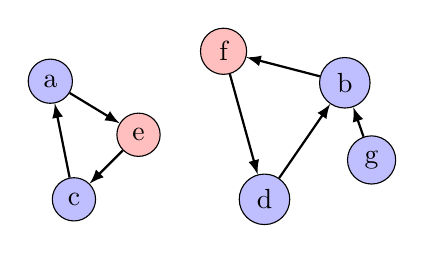
\begin{tikzpicture}
			[node/.style={circle,draw,minimum size=0.5cm,fill=blue!25!white},>=latex]
			\node[node,name=a] at (0.84,4) {a};
			\node[node,name=b]at (4.58,3.98) {b};
			\node[node,name=c]at (1.14,2.5){c};
			\node[node,name=d]at(3.56,2.5){d};
			\node[node,name=e,fill=red!25!white]at(1.96,3.32){e};
			\node[node,name=f,fill=red!25!white]at(3.04,4.38){f};
			\node[node,name=g]at(4.92,3.00){g};
			\draw[->,thick](a)--(e);
			\draw[->,thick](e)--(c);
			\draw[->,thick](c)--(a);
			\draw[->,thick](b)--(f);
			\draw[->,thick](g)--(b);
			\draw[->,thick](d)--(b);
			\draw[->,thick](f)--(d);
		\end{tikzpicture}
		\captionof{figure}{}\label{fig:grafo_orientato_cfc_trasposto}
\end{center}
\end{example}


\begin{teorbox}
		Se in un grafo orientato $G$ esiste un cammino da $u$ a $v$, allora in $G^{T}$ esiste un cammino da $v$ a $u$, e viceversa.
\end{teorbox}


\begin{corolbox}
		Se $G$ è un grafo orientato e $G^{T}$ è il grafo trasposto di $G$, allora per ogni vertice $v$ di $G$ vale:
	\begin{displaymath}
		CFC(v) = CFC^{T}(v)
	\end{displaymath}
\end{corolbox}

Dato il risultato descritto dal Teorema 3 si potrebbe pensare di applicare una DFS nel grafo $G^{T}$ a partire dalle radici $r_{i}$ degli alberi depth first ottenuti dalla DFS sul grafo $G$ in modo tale da trovare i vertici che raggiungono tali vertici $r_{i}$. Non è detto però a priori che i vertici così raggiunti appartengano alla stessa componente fortemente connessa del vertice $r_{i}$.

Infatti è possibile che la visita DFS nel grafo trasposto a partire da un vertice $r_{i}$ possa saltare da un albero depth first\footnote{Della prima visita DFS nel grafo $G$} all'altro.
Si consideri ad esempio il  grafo mostrato in Figura \ref{fig:dfs_cfc_2}. Applicando una visita in profondità a partire dal vertice $a$ si ottengono due alberi depth first  come mostrato in Figura \ref{fig:dfs_cfc_df2}:

\begin{center}
	\begin{minipage}{.45\textwidth}
		\centering
		\begin{tikzpicture}
	[node/.style={circle,draw,minimum size=0.5cm,fill=blue!25!white},>=latex]
	\node[node,fill=red!75!white,name=a]at (0.5,4){a};
	\node[node,name=b,below=0.5cm of a]{b};
	\node[node,name=c,right=1cm of b]{c};
	\node[node,name=d]at(3,4){d};
	\node[node,name=e]at(4,3){e};
	\draw[->,thick](a) --(b);
	\draw[->,thick](b)--(c);
	\draw[->,thick](c)--(a);
	\draw[->,thick](d)--(c);
	\draw[->,thick](d)--(e);
	\draw[->,thick](e)to[bend right=30](d);
	\end{tikzpicture}
\captionof{figure}{}\label{fig:dfs_cfc_2}
	\end{minipage}
\hfil
	\begin{minipage}{.45\textwidth}
		\centering
		\begin{tikzpicture}
			[node/.style={circle,draw,minimum size=0.5cm,fill=blue!25!white},>=latex]
			\node[node,name=a,fill=red!75!white]{a}
			child[->,thick]{
			node[node,name=b]{b}
			child[->,thick]{
			node[node,name=c]{c}
		}
		};
	\draw[->,thick,green](c) to[bend right =30](a);

		\node[node,name=d,fill=red!75!white,right=3cm of a]{d}
		child[->,thick]{
		node[node,name=e]{e}
	};
\draw[->,thick,green](e) to[bend right=30](d);
\draw[->,thick,green!35!black](d)to[bend right=10](c);
	\end{tikzpicture}
\captionof{figure}{}\label{fig:dfs_cfc_df2}
\end{minipage}
\end{center}

Calcolando il grafo trasposto e applicando la DFS sul vertice $a$ si ottiene un solo albero depth first che contiene due componenti fortemente connesse (vedi Figura \ref{fig:df4}).
\begin{center}
\begin{minipage}{.3\textwidth}
	\centering
		\begin{tikzpicture}
		[node/.style={circle,draw,minimum size=0.5cm,fill=blue!25!white},>=latex]
		\node[node,fill=red!75!white,name=a]at (0.5,4){a};
		\node[node,name=b,below=0.5cm of a]{b};
		\node[node,name=c,right=1cm of b]{c};
		\node[node,name=d]at(3,4){d};
		\node[node,name=e]at(4,3){e};
		\draw[->,thick](b) --(a);
		\draw[->,thick](c)--(b);
		\draw[->,thick](a)--(c);
		\draw[->,thick](c)--(d);
		\draw[->,thick](e)--(d);
		\draw[->,thick](d)to[bend left=30](e);
	\end{tikzpicture}
\captionof{figure}{Grafo trasposto}
\end{minipage}
\hfil
\begin{minipage}{.3\textwidth}
	\centering
	 	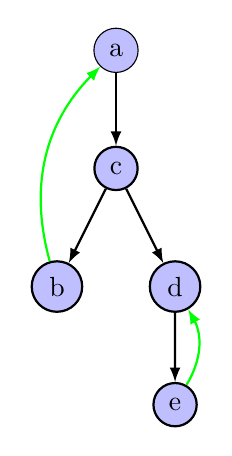
\begin{tikzpicture}
 		[node/.style={circle,draw,minimum size=0.5cm,fill=blue!25!white},>=latex]
 		\node[node,name=a]{a}
 		child[->,thick]{
 			node[node]{c}
 			child{
 				node[node,name=b]{b}
 			}
 			child{
 				node[node,name=d]{d}
 				child{
 					node[node,name=e]{e}
 				}
 			}
 		};
 	\draw[->,thick,green](e)to[bend right=30](d);
 	\draw[->,thick,green](b)to[bend left=30](a);
 	\end{tikzpicture}
 \captionof{figure}{}\label{fig:df4}
\end{minipage}
 \end{center}

La sola visita del grafo trasposto non risolve da solo il problema della mutua raggiungibilità per colpa dell'arco di attraversamento $\langle d,c\rangle$. Infatti, collegando due alberi DF diversi si stanno connettendo vertici di componenti fortemente connesse diverse\footnote{Il che è totalmente possibile ma non aiuta nel nostro tentativo di limitare la ricerca dei vertici mutualmente raggiungibili ai soli vertici di un singolo albero depth first.}. Bisogna trovare quindi un modo per inibire tali archi, fare in modo cioè che, quando la DFS (applicata sul grafo trasposto) li trova, non li segua\footnote{Non è pensabile eliminarli in quanto questo tipo di operazione altererebbe il grafo. Si ricordi, però, che nella BFS, i percorsi seguiti percorrono soltanto vertici bianchi e grigi. Basterà quindi assicurarsi che tali archi puntino a vertici neri.}.

Osserviamo innanzitutto che un arco di attraversamento, se esiste, segue sempre un verso opposto rispetto ai tempi di scoperta dei vari alberi depth first. Ovvero, dati due alberi depth first con radici in $r_{j}$ e $r_{i}$ con $j<i$, un eventuale arco di attraversamento andrà sempre all'indietro come mostrato in figura:
\begin{center}
	\begin{tikzpicture}
		[triangle/.style={isosceles triangle,draw,shape border rotate=90,isosceles triangle stretches=true, minimum height=20mm,minimum width=2cm,fill=blue!25!white},node/.style={circle,draw,minimum size=0.5cm,fill=blue!25!white},>=latex]
		\node[name=r2,right=2cm of r1]{$r_{1}$};
		\node[triangle,anchor=north] at (r2.south){};
		\node[name=r3,right=2cm of r2]{$r_{2}$};
		\node[triangle,anchor=north] at (r3.south){};
		\node[name=r4,right=2cm of r3]{$r_{3}$};
		\node[triangle,anchor=north] at (r4.south){};
		\node[name=r5,right=2cm of r4]{$r_{4}$};
		\node[triangle,anchor=north,name=t5] at (r5.south){};
		\node[anchor=west,right=1cm of t5.center]{$\ldots$};
		\node[name=r6,right=2cm of r5]{$r_{k-1}$};
		\node[triangle,anchor=north,name=t6] at (r6.south){};
		\node[name=r7,right=2cm of r6]{$r_{k}$};
		\node[triangle,anchor=north,name=t7] at (r7.south){};
		\node[node,name=b,fill=white]at(t7.center){};
		\node[node,name=n,fill=black]at(t6.center){};
		\draw[->,thick,green!35!black](b)to[bend right=30](n);
		\draw[->,thick](2,-3)--(17,-3)node[anchor=north]{Tempo};
	\end{tikzpicture}
\captionof{figure}{Foresta depth first generata da una visita in profondità su un grafo}\label{fig:arco_attraversamento}
\end{center}
Ovviamente, se nel grafo $G$ gli archi di attraversamento collegano alberi nuovi ad alberi vecchi, eseguendo una visita in profondità sul grafo trasposto si avrà un'inversione della direzione di tali archi (che andranno quindi da alberi depth first vecchi ad alberi depth first nuovi).

\begin{center}
	\begin{tikzpicture}
		[triangle/.style={isosceles triangle,draw,shape border rotate=90,isosceles triangle stretches=true, minimum height=20mm,minimum width=2cm,fill=pink!25!white},node/.style={circle,draw,minimum size=0.5cm,fill=blue!25!white},>=latex]
		\node[name=r2,right=2cm of r1]{$r_{1}$};
		\node[triangle,anchor=north] at (r2.south){};
		\node[name=r3,right=2cm of r2]{$r_{2}$};
		\node[triangle,anchor=north] at (r3.south){};
		\node[name=r4,right=2cm of r3]{$r_{3}$};
		\node[triangle,anchor=north] at (r4.south){};
		\node[name=r5,right=2cm of r4]{$r_{4}$};
		\node[triangle,anchor=north,name=t5] at (r5.south){};
		\node[anchor=west,right=1cm of t5.center]{$\ldots$};
		\node[name=r6,right=2cm of r5]{$r_{k-1}$};
		\node[triangle,anchor=north,name=t6] at (r6.south){};
		\node[name=r7,right=2cm of r6]{$r_{k}$};
		\node[triangle,anchor=north,name=t7] at (r7.south){};
		\node[node,name=b,fill=white]at(t7.center){};
		\node[node,name=n,fill=black]at(t6.center){};
		\draw[->,thick,green!35!black](n)to[bend left=30](b);
		\draw[->,thick](2,-3)--(17,-3)node[anchor=north]{Tempo};
	\end{tikzpicture}
	\captionof{figure}{Direzione degli archi di attraversamento nel grafo trasposto}
\end{center}

Al termine dell'esplorazione di tutti i vertici bianchi raggiungibili da una sorgente $s$, l'Algoritmo \textsc{DFS\_Visit}$(G,s)$ (Algoritmo \ref{lst:dfs_visit_graph}) lo colora di nero. Questo significa quindi che un arco di attraversamento come mostrato nella Figura \ref{fig:arco_attraversamento} va sempre da vertici colorati di bianco a vertici colorati di nero\footnote{Questo in quanto gli alberi $T_{r_{k}}$ vengono costruiti sempre e solo dopo la terminazione della costruzione dell'albero $T_{r_{k-1}}$.}. Chiaramente, nel caso di una DFS nel grafo trasposto l'esatto contrario: un arco di attraversamento collega sempre un vertice nero ad un vertice bianco.

\begin{center}
	\begin{tikzpicture}
		[triangle/.style={isosceles triangle,draw,shape border rotate=90,isosceles triangle stretches=true, minimum height=20mm,minimum width=2cm,fill=pink!25!white},node/.style={circle,draw,minimum size=0.5cm,fill=blue!25!white},>=latex]
		\node[name=r2,right=2cm of r1]{$r_{1}$};
		\node[triangle,anchor=north] at (r2.south){};
		\node[name=r3,right=2cm of r2]{$r_{2}$};
		\node[triangle,anchor=north] at (r3.south){};
		\node[name=r4,right=2cm of r3]{$r_{3}$};
		\node[triangle,anchor=north] at (r4.south){};
		\node[name=r5,right=2cm of r4]{$r_{4}$};
		\node[triangle,anchor=north,name=t5] at (r5.south){};
		\node[anchor=west,right=1cm of t5.center]{$\ldots$};
		\node[name=r6,right=2cm of r5]{$r_{k-1}$};
		\node[triangle,anchor=north,name=t6] at (r6.south){};
		\node[name=r7,right=2cm of r6]{$r_{k}$};
		\node[triangle,anchor=north,name=t7,fill=black!50] at (r7.south){};
		\node[node,name=n,fill=white]at(t6.center){};
		\draw[->,thick,green!35!black](n)to[bend left=30](t7.center);
		\draw[->,thick](2,-3)--(17,-3)node[anchor=north]{Tempo};
	\end{tikzpicture}
	\captionof{figure}{}
\end{center}

Prendiamo quindi l'albero $T_{r_{k}}$ e consideriamo di eseguire una DFS applicata sul grafo trasposto. Chiaramente, essendo tale albero l'ultimo costruito nella prima DFS, non possono esistere altri alberi in cui un eventuale arco di attraversamento possa puntare andando in avanti. Per questo motivo l'applicazione dell'Algoritmo \textsc{DFS\_Visit}$(G^{T},r_{k})$ può solo raggiungere vertici dell'albero $T_{r_{k}}$. Terminata tale procedura tutti i vertici (per semplicità) di $T_{r_{k}}$ saranno colorati di nero. A questo punto \textsc{DFS\_Visit}$(G^{T},r_{k-1})$ vedrà inibiti gli archi di attraversamento che puntano a $T_{r_{k}}$.

Essendo l'albero $T_{r_{k}}$ l'ultimo albero della foresta depth first ottenuta nella prima DFS si avrà che il vertice $r_{k}$ sarà il vertice che avrà il massimo tempo di fine visita, sarà ovvero l'ultimo vertice ad essere eliminato dallo stack. Per inibire, quindi, gli archi di attraversamento sarà sufficiente eseguire l'algoritmo \textsc{DFS\_Visit} selezionando i vertici in ordine inverso rispetto ai tempi di fine visita ottenuti nella prima DFS.

Possiamo dunque pensare di modificare l'Algoritmo DFS in modo tale da salvare in uno stack i vertici in ordine di tempo di fine visita. In questo modo, una volta terminata la prima DFS, sarà sufficiente eseguire una seconda DFS sul grafo trasposto in ordine inverso rispetto ai tempi di fine visita ottenuti nella prima DFS. Ogni albero depth first ottenuto in questa seconda visita corrisponderà ad una componente fortemente connessa del grafo $G$.

\begin{minipage}{.45\textwidth}
	\begin{lstlisting}[caption={\textsc{DFS}(G)}, label={lst:dfs_cfc},language=asd]
S = @$\emptyset$@
Init(G)
for each v @$\in$@ V do
	if Color[v] = White then
		S = DFS_Visit(G,v,S)
return S
\end{lstlisting}
\end{minipage}
\hfil
\begin{minipage}{.45\textwidth}
	\begin{lstlisting}[caption={\textsc{DFS\_Visit}(G,v,S)}, label={lst:dfs_visit_cfc},language=asd]
Color[v] = Gray
for each u @$\in$@ Adj[v] do
	if Color[u] = White then
		S = DFS_Visit(G,u,S)
S = Push(S,v)
Color[v] = Black
return S
\end{lstlisting}
\end{minipage}

\begin{minipage}{.45\textwidth}
	\begin{lstlisting}[caption={\textsc{DFS2}($G^{T}$,S)},language=asd]
Init(@$G^{T}$@)
while (S @$\neq \emptyset$@)
	v = Top(S)
	if Color[v] = White then
		DFS_Visit2(@$G^{T}$@,v)
	S = Pop(S)
\end{lstlisting}
\end{minipage}
\hfil
\begin{minipage}{.45\textwidth}
	\begin{lstlisting}[caption={\textsc{DFS\_Visit2}($G^{T}$,v)},language=asd]
	Color[v] = Gray
	for each u @$\in$@ Adj[v] do
		if Color[u] = White then
			Pred[u] = v
			DFS_Visit2(@$G^{T}$@,u)
\end{lstlisting}
\end{minipage}

\begin{lstlisting}[caption={\textsc{CFC}(G)},language=asd]
S = DFS(G)
@$G^{T}$@ = GrafoTrasposto(G)
DFS2(@$G^{T}$@ ,S)
\end{lstlisting}

Il calcolo del grafo trasposto si può ottenere calcolando la matrice trasposta della matrice di adiacenza oppure, nel caso delle liste di adiacenza costruendo delle nuove liste a partire da quelle del grafo $G$:
\begin{lstlisting}[caption={\textsc{GrafoTrasposto}(G)},language=asd]
@$V^{T}$@  = @$\emptyset$@
for each v  @$\in$@ V
	@$V^{T}$@ = @$V^{T}$@  @$\cup$@ {v}
for each v @$\in$@ V do
	for each u @$\in$@ Adj[v] do
		@$Adj^{T}$@[u] = InserisciInTesta(@$Adj^{T}$@[u],v)
return (@$V^{T},Adj^{T}$@)
\end{lstlisting}
È immediato osservare che l'algoritmo \textsc{CFC}$(G)$ ha una complessità lineare sulla dimensione del grafo $G$.

\section{Cammini minimi nei grafi}
Lo studente Ciro Esposito deve andare a sostenere lo scritto di Algoritmi e Strutture Dati che si terrà in un'aula della sede di Ingegneria a Piazzale Tecchio ma come al solito la Circumvesuviana lo ha fatto fare tardi. Non appena arrivato alla stazione centrale di Napoli si pone il problema di trovare la strada più corta possibile dalla stazione a Fuorigrotta e così apre Google Maps per vedere i vari percorsi disponibili e cercare quello più breve.

Come mostrato in Figura \ref{fig:maps} l'applicazione associa a ciascun percorso un tempo di percorrenza ottenuto sommando i tempi di percorrenza necessari ad attraversare i vari punti lungo il percorso. Riuscirà il nostro studente ad arrivare in tempo?
\begin{center}
	\includegraphics[scale=.45]{res/Maps}
	\captionof{figure}{I possibili percorsi per raggiungere la sede di Piazzale Tecchio a partire dalla stazione Centrale di Napoli}\label{fig:maps}
\end{center}

\subsection{I grafi pesati}
Per risolvere questa tipologia di problema che attanaglia migliaia di studenti ritardatari si fa uso del concetto di \textbf{grafo pesato}.

\dfn{Grafo pesato}{
	Un \textbf{grafo pesato} è una grafo orientato $G=(V,E,w)$ in cui a ciascun arco viene associato un \textbf{peso} di valore reale espresso dalla funzione:
	\begin{equation}
		w : E \longrightarrow \mathbb{R}
	\end{equation}
}

Dato un percorso $\pi = \langle v_{0},v_{1},\ldots, v_{k} \rangle$ è possibile considerare il \textbf{peso} $w(\pi)$ di tale percorso ottenuto sommando i pesi degli archi che compongono $\pi$:
\begin{equation}
	w(\pi) = \sum_{i=1}^{k} w(v_{i-1},v_{i})
\end{equation}

La ricerca del percorso minimo equivale quindi alla ricerca del percorso che minimizzi la quantità $w(\pi)$.

\dfn{Cammino minimo}{
	Il \textbf{peso di un cammino minimo} $\delta(u,v)$ da $u$ a $v$ è definito come:
	\begin{equation}
		\delta(u,v) = \begin{cases}
			min \{w(\pi): u \stackrel{\pi}{\leadsto} v\} & \text{Se esiste un cammino da $u$ a $v$}\\
			\infty & \text{Altrimenti}
		\end{cases}
	\end{equation}
	Un \textbf{cammino minimo} dal vertice $u$ al vertice $v$ è definito come un cammino qualsiasi $\pi$ con peso $w(\pi)=\delta(u,v)$.
}

In questa sezione ci occuperemo dell'analisi del \textbf{problema dei cammini minimi da sorgente unica}: dato un grafo $G=(V,E,w)$, vogliamo trovare un cammino minimo che va da un dato vertice \textbf{sorgente} $s \in V$ a ciascun vertice $v \in V$.

Poiché la funzione $w$ è una funzione a valori reali, in alcuni casi del problema dei cammini minimi da sorgente unica possono presentarsi degli archi in cui i pesi sono negativi. Se il grafo $G=(V,E)$ non contiene cicli di peso negativo che sono raggiungibili dalla sorgente $s$, allora per ogni $v \in V$, il peso del cammino minimo $\delta(s,v)$ resta ben definito, anche se ha un valore negativo. Tuttavia, se esiste un ciclo di peso negativo che è raggiungibile da $s$, i pesi dei cammini minimi non sono ben definiti. Nessun cammino da $s$ ad un vertice del ciclo può essere un cammino minimo in quanto è sempre possibile trovare un cammino di peso minore che segue il cammino ``minimo'' proposto e poi attraversare il ciclo di peso negativo.


\begin{osservation}
		Se il grafo ha pesi negativi e ci sono cicli (rispetto ad una sorgente) il percorso minimo \textbf{non esiste}.
\end{osservation}


\begin{example}
	Consideriamo il seguente grafo pesato:
	\begin{center}
		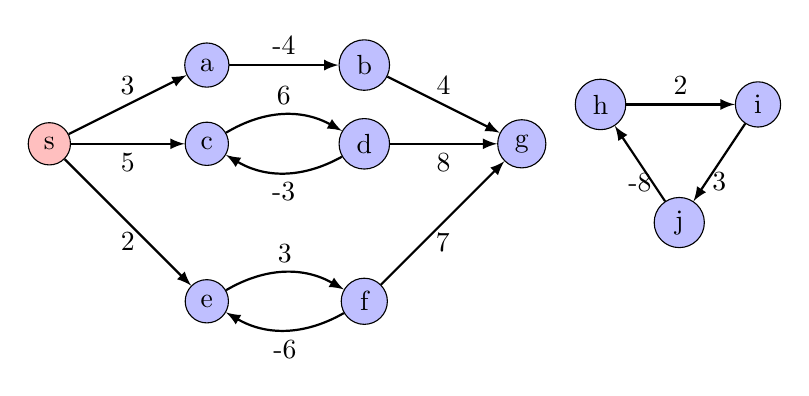
\begin{tikzpicture}
			[node/.style={circle,draw,minimum size=0.5cm,fill=blue!25!white},>=latex]
			\node[node,name=s,fill=red!25!white]at(-1,1){s};
			\node[node,name=a]at(1,2){a};
			\node[node,name=b]at(3,2){b};
			\node[node,name=c]at(1,1){c};
			\node[node,name=d]at(3,1){d};
			\node[node,name=g]at(5,1){g};
			\node[node,name=e]at(1,-1){e};
			\node[node,name=f]at(3,-1){f};
			\node[node,name=i]at(8,1.5){i};
			\node[node,name=h]at(6,1.5){h};
			\node[node,name=j]at(7,0){j};
			\draw[->,thick](s)--node[midway,above]{3}(a);
			\draw[->,thick](a)--node[midway,above]{-4}(b);
			\draw[->,thick](b)--node[midway,above]{4}(g);
			\draw[->,thick](f)--node[midway,below]{7}(g);
			\draw[->,thick](s)--node[midway,below]{2}(e);
			\draw[->,thick](s)--node[midway,below]{5}(c);
			\draw[->,thick](d)--node[midway,below]{8}(g);
			\draw[->,thick](h)--node[midway,above]{2}(i);
			\draw[->,thick](j)--node[midway,below]{-8}(h);
			\draw[->,thick](i)--node[midway,below]{3}(j);
			\draw[->,thick](c)to[bend left=30]node[midway,above]{6}(d);
			\draw[->,thick](d)to[bend left=30]node[midway,below]{-3}(c);
			\draw[->,thick](f)to[bend left=30]node[midway,below]{-6}(e);
			\draw[->,thick](e)to[bend left=30]node[midway,above]{3}(f);
		\end{tikzpicture}
	\end{center}
Se volessimo calcolare un percorso minimo dalla sorgente $s$ al vertice $f$ notiamo l'esistenza di un ciclo di peso negativo. Infatti, calcolando il peso dei vari percorsi possibili si osserva che non esiste un possibile percorso minimo:
\begin{displaymath}
	\begin{array}{l}
		w(\langle s,e,f \rangle) = 2+3 = 5\\
		w(\langle s,e,f,e,f \rangle) = 5+(-6)+3 = 2\\
		w(\langle s,e,f,e,f,e,f \rangle) = 2 + (-6) +3 =-1
	\end{array}
\end{displaymath}
Alcuni algoritmi per cammini minimi, come l'Algoritmo di Dijkstra, suppongono che tutti i pesi degli archi del grafo di input siano non negativi. Altri, come l'Algoritmo di Bellman-Ford, accettano archi di peso negativo nel grafo di input a patto di non avere cicli di peso negativo raggiungibili dalla sorgente.
\end{example}

\begin{example}
	Come abbiamo appena visto, un cammino minimo non può avere un ciclo di peso negativo. Non può avere nemmeno un ciclo di peso positivo, perché eliminando il ciclo dal cammino si ottiene un cammino con la stessa sorgente, la stessa direzione e un peso più piccolo.
	\medskip

	Se $\pi=\langle v_{0},v_{1},v_{2},\ldots,v_{k}\rangle$ è un cammino e $\xi = \langle v_{i}, v_{i+1}, \ldots, v_{j} \rangle $ è un ciclo di peso positivo in questo cammino (cosicché $v_{i}=v_{j}$ e $w(\xi)>0$), allora il cammino $\pi' = \langle v_{0},v_{1},\ldots,v_{i},v_{j+1},v_{j+2},\ldots,v_{k} \rangle$ ha peso $w(\pi')=w(\pi)-w(c)<w(\pi)$, e quindi $\pi$ non può essere un cammino minimo da $v_{0}$ a $v_{k}$.
\end{example}

\subsection{Il rilassamento}
Gli algoritmi descritti in questa sezione usano la tecnica del \textbf{rilassamento} (vedi Figura \ref{fig:relax}) Per ogni vertice $v \in V$ conserviamo in un array:
\begin{equation}
	d : V \longrightarrow \mathbb{R}
\end{equation}
le stime dei vari percorsi minimi a partire da un vertice sorgente $s$ : $\delta(s,v)$. L'attributo $d[v]$ è detto \textbf{stima del cammino minimo}. Il processo di rilassamento di un arco $(u,v)$ consiste nel verificare se, passando per un vertice $u$, è possibile migliorare il cammino minimo per arrivare a $v$ precedentemente trovato e, in tal caso, aggiornare i valori $d[v]$ e $pred[v]$. Può essere visto come un rilassamento del vincolo:
\begin{equation}\label{eq:relax}
	d[v] \leq d[u] + w(u,v)
\end{equation}
che, per disuguaglianza triangolare deve essere soddisfatto se:
\begin{displaymath}
	\begin{array}{l}
		d[u] = \delta(s,u)\\
		d[v] = \delta(s,v)
	\end{array}
\end{displaymath}
Ovvero, se $d[u] \leq d[u] + w(u,v)$ non occorre esercitare alcuna ``pressione'' affinché il vincolo \ref{eq:relax} sia rispettato. L'effetto di un passo di rilassamento può ridurre il valore della stima del cammino minimo $d[v]$ e aggiornare il campo $pred[v]$ del predecessore di $v$. L'esecuzione del passo di rilassamento viene eseguito a tempo costante.
\begin{lstlisting}[caption={\textsc{Relax}(u,v,w)},language=asd]
if d[v] > d[u]+w(u,v)
	d[v] = d[u] +w(u,v)
	pred[v] = u
\end{lstlisting}

\subsection{Proprietà dei cammini minimi e del rilassamento}


\begin{lemmabox}
		Sia $G=(V,E,w)$ un grafo pesato e $\pi = \langle v_{1}, v_{2}, v_{3}, \ldots, v_{k-1}, v_{k} \rangle $ un percorso minimo da $v_{1}$ a $v_{k}$. Per ogni coppia $(i,j)$ tale che $1 \leq i < j \leq k$ allora il sottopercorso di $\pi$:
	\[\pi_{i,j}= \langle v_{i},v_{i+1},\ldots,v_{j}\rangle\]
	è un percorso minimo da $v_{i}$ a $v_{j}$, $\pi_{i,j}$ prende il nome di \textbf{grafo infisso} del percorso $\pi$.
\end{lemmabox}
\begin{proof}
	Se scomponiamo il cammino $\pi$ in:
\begin{displaymath}
	v_{0} \stackrel{\pi_{0i}}{\leadsto} v_{i} \stackrel{\pi_{ij}}{\leadsto} v_{j} \stackrel{\pi_{jk}}{\leadsto}v_{k}
\end{displaymath}
allora abbiamo:
\begin{align*}
	w(\pi) & = w(\pi_{0i} ) + w(\pi_{ij}) + w(\pi_{jk}) = \\
	&= \sum_{z=1}^{i-1} w(v_{z},v_{z+1}) + \sum_{z=i}^{j-1}w(v_{z},v_{z+1}) + \sum_{z=j}^{k-1}w(v_{z},v_{z+1})
\end{align*}
Supponiamo adesso che ci sia un percorso $\pi'_{ij}$ da $v_{i}$ a $v_{j}$ con peso $w(\pi'_{ij})<w(\pi_{ij})$. Allora il cammino $\pi'$:
\[v_{0} \stackrel{\pi_{0i}}{\leadsto} v_{i} \stackrel{\pi'_{ij}}{\leadsto} v_{j} \stackrel{\pi_{jk}}{\leadsto}v_{k}\] è un cammino da $v_{0}$  a $v_{k}$ il cui peso:
\begin{align*}
	w(\pi') & = w(\pi_{0i} ) +\underbrace{ w(\pi'_{ij})}_{<w(\pi_{ij})} + w(\pi_{jk}) < w(\pi_{0i} ) + w(\pi_{ij}) + w(\pi_{jk}) = w(\pi)
\end{align*}
è minore di $w(\pi)$ che contraddice l'ipotesi secondo la quale $\pi$ sia un cammino minimo da $v_{0}$ a $v_{k}$.
\end{proof}

\begin{corolbox}
		Dato $G=(V,E,w)$ e $\pi=\langle v_{1},v_{2},\ldots,v_{k-1},v_{k}\rangle$ un percorso minimo da $v_{1}$ a $v_{k}$ allora:
	\begin{equation}
		\delta(v_{1},v_{k}) = \delta(v_{1},v_{k-1}) + w(v_{k-1},v_{k})
	\end{equation}
\end{corolbox}

\begin{proof}
	Possiamo pensare di scomporre $\pi$ come segue:
\begin{displaymath}
	\pi = v_{1} \stackrel{\pi_{1,k-1}}{\leadsto}v_{k-1} \leadsto v_{k}
\end{displaymath}
e per il Lemma 1 il percorso $\pi_{1,k-1}$ risulta minimo. Quindi:
\begin{displaymath}
	w(\pi_{1,k-1}) = \delta(v_{1},v_{k-1})
\end{displaymath} da cui segue l'asserto.
\end{proof}

\begin{lemmabox}[Disuguaglianza triangolare]
	Dato $G=(V,E,w)$ e $s \in V$, per ogni arco $(u,v) \in E$ vale:
	\begin{equation}
		\delta(s,v) \leq \delta(s,u) + w(u,v)
	\end{equation}
\end{lemmabox}


\begin{lemmabox}
		Dato $G=(V,E,w)$ e $(u,v) \in E$, immediatamente dopo l'esecuzione dell'Algoritmo \textsc{Relax}$(u,v,w)$ varrà che:
	\begin{displaymath}
		d[v] \leq d[u] + w(u,v)
	\end{displaymath}
\end{lemmabox}

\begin{proof}
	Immediata per come è scritto l'algoritmo.
\end{proof}

\begin{figure}[ht!]
\centering
\subfloat[\label{fig:relax1}]{	\begin{tikzpicture}
		[node/.style={circle,draw,minimum size=0.5cm,fill=blue!25!white},>=latex]
		\node[node,name=u1]at(0,0){5};
		\node[node,name=v1,right=2cm of u1]{9};
		\node[node,name=u2,below=1cm of u1]{5};
		\node[node,name=v2,below=1cm of v1]{7};
		\node[anchor=south]at(u1.north){u};
		\node[anchor=south]at(u2.north){u};
		\node[anchor=south]at(v1.north){v};
		\node[anchor=south]at(v2.north){v};
		\draw[->,thick](u1) --node[midway,above]{2}(v1);
		\draw[->,thick](u2) --node[midway,above]{2}(v2);
 		\draw[->,dashed,line width=2pt] (1,-0.2) to node[midway,xshift=1.5cm]{\textsc{Relax}$(u,v,w)$} (1,-1.2);
	\end{tikzpicture}} \hfil
\subfloat[\label{fig:relax2}]{	\begin{tikzpicture}
		[node/.style={circle,draw,minimum size=0.5cm,fill=blue!25!white},>=latex]
		\node[node,name=u1]at(0,0){5};
		\node[node,name=v1,right=2cm of u1]{6};
		\node[node,name=u2,below=1cm of u1]{5};
		\node[node,name=v2,below=1cm of v1]{6};
		\node[anchor=south]at(u1.north){u};
		\node[anchor=south]at(u2.north){u};
		\node[anchor=south]at(v1.north){v};
		\node[anchor=south]at(v2.north){v};
		\draw[->,thick](u1) --node[midway,above]{2}(v1);
		\draw[->,thick](u2) --node[midway,above]{2}(v2);
		\draw[->,dashed,line width=2pt] (1,-0.2) to node[midway,xshift=1.5cm]{\textsc{Relax}$(u,v,w)$} (1,-1.2);
\end{tikzpicture}}
\caption{Rilassamento dell'arco $(u,v)$ con peso $w(u,v) = 2$. La stima del cammino minimo è illustrata all'interno del vertice. \textbf{(\ref{fig:relax1})} Poiché $v[d]>d[v]+w(u,v)$, il valore $d[v]$ diminuisce.\textbf{(\ref{fig:relax2})} Qui, $d[v] \leq d[u] + w(u,v)$ prima del rilassamento quindi \textsc{Relax}$(u,v,w)$ non modifica la stima. }\label{fig:relax}
\end{figure}


\begin{lemmabox}
	Dato $G=(V,E,w)$ e posto\footnote{Nei grafi non pesati l'algoritmo \textsc{Init} inizializzava le distanze a $\infty$ poiché non si sapeva nulla a priori sulla raggiungibilità dei vertici e $d[s]=0$. Anche nei grafi pesati è corretto inizializzare $d[s]=0$ in quanto ci sarebbe altrimenti un ciclo negativo che impedisce l'esistenza dei percorsi minimi.}:
\begin{displaymath}
	\begin{array}{l}
		\forall v \in V \setminus \{s\} (d[v] = \infty) \\
		d[s] = 0
	\end{array}
\end{displaymath}
lungo una qualsiasi sequenza di operazioni di rilassamento vale sempre:
\begin{displaymath}
	\forall v \in V (d[v]  \geq \delta(s,v) )
\end{displaymath}
\end{lemmabox}

\begin{proof}
	Si dimostra per induzione sul numero $i$ delle operazioni di rilassamento.
\begin{itemize}
	\item \textbf{Caso base:}  Sia $i=0$. Non è stata eseguita alcuna operazione di rilassamento quindi la proprietà risulta vera per come sono stati inizializzati i vertici.
	\item \textbf{Passo induttivo:} Sia $i>0$, ciò significa che è stata eseguita almeno una operazione di rilassamento. Supponiamo vero l'asserto prima della $i$-esima operazione di rilassamento. Si consideri l'arco $(x,y) \in E$ ed eseguiamo l'operazione \textsc{Relax}$(x,y,w)$ che andrà a modificare la stima di $y$. Sicuramente vale:
	\begin{displaymath}
		\forall v \in V\setminus\{y\} \bigl(d[v] \geq \delta(s,v)\bigr)
	\end{displaymath}
Consideriamo quindi i due casi:
\begin{enumerate}
	\item \textbf{Caso 1:} se prima dell'operazione di relax vale $d[y] \leq d[x] + w(x,y)$ allora $d[y] \geq \delta(s,y)$
	\item \textbf{Caso 2:} se prima dell'operazione di relax vale $d[y] > d[x] + w(x,y)$ allora si pone $d[y] = d[x] +w(x,y)$. Prima di tale operazione ovviamente valeva $d[x] \geq \delta(s,x)$ per ipotesi induttiva. Per il Lemma 2 si ha $\delta(s,y) \leq \delta(s,x)+w(x,y)$. Sommando entrambi i membri per la stessa quantità si ha:
	\begin{displaymath}
		d[x] + w(x,y) \geq \delta(s,x)+w(x,y) \geq \delta(s,y)
	\end{displaymath}
Quindi: \[ d[y] = d[x] + w(x,y) \geq \delta(s,y) \]
\end{enumerate}
\end{itemize}
\end{proof}


\begin{corolbox}
	Se non c'è un cammino da $s$ a $v$ allora si ha sempre $d[v] = \delta(s,v) = \infty$.
\end{corolbox}

\begin{proof}
	Ovvia dalla precedente. Se un vertice $v$ non è raggiungibile da $s$ allora si avrà in ogni momento $d[v] \geq \delta(s,v)$ e non può essere meno di $\infty$. Per questo motivo l'algoritmo di rilassamento è corretto sui vertici non raggiungibili.
\end{proof}


\begin{lemmabox}
		Dato $G=(V,E,w)$ e $s \in V$ e sia $\pi = \langle v_{1}, v_{2}, \ldots,v_{k-1}, v_{k} \rangle$ un percorso minimo da $v_{1}=s$ a $v_{k}$.Inizializzando $d[v_{i}] = \infty$ per ogni $1<i\leq k$ e $d[s]=0$ e presa una sequenza arbitraria di rilassamenti che contiene \textsc{Relax}$(v_{k-1},v_{k},w)$ (l'ultimo arco del percorso $\pi$), se prima di tale rilassamento valeva:
	\begin{displaymath}
		d[v_{k-1}] = \delta(s,v_{k-1})
	\end{displaymath}
allora dopo tale passo varrà:
\begin{displaymath}
	d[v_{k}] = \delta(s,v_{k})
\end{displaymath}
\end{lemmabox}

\begin{proof}
	Consideriamo una retta orientata sulla quale vengono disposti i passi di rilassamento applicati sul percorso $\pi$:
\begin{center}
	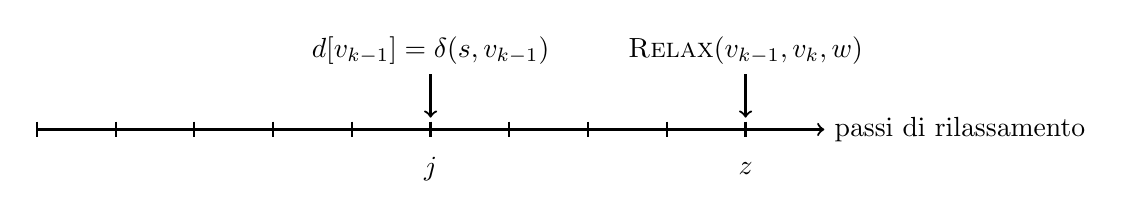
\begin{tikzpicture}
		\draw[->, thick] (-5,0)--(5,0) node[right]{passi di rilassamento};
		\foreach \i in {-5,...,4}
		\draw[thick] (\i,.1)--(\i,-.1) node[below]{};
		\node[]at(0,-.5){$j$};
		\node[]at(4,-.5){$z$};
		\node[name=a]at(0,1){$d[v_{k-1}]=\delta(s,v_{k-1})$};
		\draw[->,thick](a) -- (0,.15);
		\node[name=b]at(4,1){\textsc{Relax}$(v_{k-1},v_{k},w)$};
		\draw[->,thick](b) -- (4,.15);
	\end{tikzpicture}
\end{center}
Vorremmo assicurarsi che anche prima della $z$-esima operazione valga ancora $d[v_{k-1}] = \delta(s,v_{k-1})$. Chiaramente questo è  assicurato dal modo in cui abbiamo implementato l'algoritmo di rilassamento. Infatti, per il Lemma 4 tale quantità può solo aumentare ma se diventa più grande il passo di rilassamento non lo modificherà. Si hanno quindi i seguenti casi:
\begin{enumerate}
	\item \textbf{Caso 1:} si ha \[d[v_{k}]\leq d[v_{k-1}]+w(v_{k-1},v_{k}) = \delta(s,v_{k-1}) + w(v_{k-1},v_{k}) \]
	Per il Corollario 1:
	\begin{align*}
		\delta(s,v_{k}) &= \delta(s,v_{k-1}) + w(v_{k-1},v_{k})\\
		&= \delta(s,v_{k}) & \text{\textcolor{gray}{Per il Lemma 4}}
	\end{align*}
\item \textbf{Caso 2:} Se $d[v_{k}]> d[v_{k-1}]+w(v_{k-1},v_{k})$ allora:
\begin{align*}
	d[v_{k}] &= d[v_{k-1}]+w(v_{k-1},v_{k})\\
	&= \delta(s,v_{k-1}) + w(v_{k-1},v_{k}) & \text{\textcolor{gray}{Per ipotesi}}\\
	&= \delta(s,v_{k}) & \text{\textcolor{gray}{Per Corollario 1}}
\end{align*}
\end{enumerate}
\end{proof}

\subsection{L'algoritmo di Bellman-Ford}
L'algoritmo di Bellman-Ford (Algoritmo \ref{lst:bellman-ford}) risolve il problema dei cammini minimi da sorgente unica nel caso generale in cui i pesi degli archi possono essere negativi. Dato un grafo orientato $G=(V,E,w)$ con sorgente $s \in V$, l'algoritmo di Bellman-Ford restituisce un valore booleano che indica se esiste oppure no un ciclo di peso negativo che è raggiungibile dalla sorgente. Se un tale ciclo esiste, l'algoritmo indica che il problema non ha soluzione. Se un tale ciclo non esiste, l'algoritmo fornisce i cammini minimi e i loro pesi.

L'Algoritmo usa il rilassamento, riducendo progressivamente il valore stimato $d[v]$ per il peso di un cammino minimo dalla sorgente $s$ a ciascun vertice $v \in V$, fino a raggiungere il peso effettivo $\delta(s,v)$ di un cammino minimo.
\begin{lstlisting}[caption={\textsc{Init}(G,s)},language=asd]
	for each v @$\in$@ V do
		d[v] = @$\infty$@
		d[s] = 0
\end{lstlisting}
\begin{lstlisting}[caption={\textsc{Bellman-Ford}(G,w,s)},language=asd,label=lst:bellman-ford]
	Init(G,s)
	for i = 1 to |V|-1 do
		for each (u,v) @$\in$@ E do
			Relax(u,v,w)
	for each (u,v) @$\in$@ E do
		if d[v] > d[u] + w(u,v) then
			return false
	return true
\end{lstlisting}
L'algoritmo di Bellman-Ford viene eseguito nel tempo $O(VE)$ perché l'inizializzazione richiede un tempo $\Theta(V)$, ciascuno dei $|V|-1$ passaggi sugli arghi nelle righe 2-4 richiede un tempo $\Theta(E)$ e il ciclo \texttt{for} nelle righe 5-7 richiede un tempo $O(E)$.

\subsubsection{Correttezza di Bellman-Ford}


\begin{lemmabox}
	Sia $G=(V,E,w)$ un grafo orientato pesato con sorgente $s$. Supponiamo che $G$ non contenga cicli di peso negativo che sono raggiungibili da $s$. Allora, dopo $|V|-1$ iterazioni del ciclo \texttt{for} delle righe 2-4 di \textsc{Bellman-Ford}, si ha $v[d] = \delta(s,v)$ per tutti i vertici che sono raggiungibili da $s$.
\end{lemmabox}

\begin{proof}
	Sia $v$ un qualsiasi vertice raggiungibile da $s$ e sia $\pi = \langle v_{0}, v_{1}, v_{2}, v_{3}, \ldots, v_{k-1}, v_{k} \rangle$, dove $v_{0}=s$ e $v_{k}=v$, un percorso minimo da $s$ a $v$. Tale cammino essendo minimo e aciclico avrà al massimo $|V|-1$ archi, quindi $k \leq |V| -1$. Ciascuna delle $|V|-1$ iterazioni del ciclo \texttt{for} delle righe 2-4 rilassa tutti gli $|E|$ archi. Fra gli archi rilassati nella $i$-esima iterazione, per $i=1,2,\ldots,k$, c'è l'arco $(v_{i-1},v_{i})$. Per il Lemma 5 si avrà quindi $d[v]=d[v_{k}]=\delta(s,v_{k})=\delta(s,v)$. 
\end{proof}


\begin{corolbox}
	Sia $G=(V,E,w)$ un grafo orientato pesato con sorgente $s$. Per ogni vertice $v \in V$, esiste un cammino da $s$ a $v$ se e soltato se l'algoritmo \textsc{Bellman-Ford} termina con $d[v]<\infty$ quando viene eseguito sul grafo $G$.
\end{corolbox}

\begin{teorbox}[Correttezza di \textsc{Bellman-Ford}]
Supponiamo di eseguire l'algoritmo di \textsc{Bellman-Ford} su un grafo orientato pesato con sorgente $s$. Se  $G$ non contiene cicli di peso negativo che sono raggiungibili da $s$, allora l'algoritmo restituisce \textsc{true}, si ha $v[d]= \delta(s,v)$ per tutti i vertici $v \in V$. Se $G$ contiene un ciclo di peso negativo che è raggiungibile da $s$ allora l'algoritmo restituisce \textsc{false}.
\end{teorbox}

\begin{proof}
	Supponiamo che il grafo $G$ non abbia cicli di peso negativo raggiungibili dalla sorgente $s$. Per ogni vertice $v$ raggiungibile da $s$ il Lemma 6 assicura che, al termine dell'algoritmo, vale $d[v]=\delta(s,v)$. Se $v$ non è raggiungibile da $s$ allora l'asserzione è vera per il Corollario 2.

Al termine dell'algoritmo, per tutti gli archi $(u,v) \in E$ si ha:
\begin{align*}
	v[d] &= \delta(s,v)\\
		&= \delta(s,u) + w(u,v) & \text{\textcolor{gray}{(Per la disuguaglianza triangolare)}}\\
		&= d[u] + w(u,v)
\end{align*}
Quindi nessuno dei controlli fa sì che l'algoritmo di \textsc{Bellman-Ford} restituisca \textsc{false}, quindi l'algoritmo restituisce \textsc{true}.

Supponiamo che il grafo $G$ contenga un ciclo di peso negativo che è raggiungibile dalla sorgente $s$, indichiamo questo ciclo con $\xi = \langle v_{0},v_{1},v_{2},\ldots,v_{k} \rangle$, dove $v_{0}=v_{k}$. Allora:
\begin{equation}\label{eq:bellman}
	\sum_{i=1}^{k}w(v_{i-1},v_{i})<0
\end{equation}
Supponiamo per assurdo che l'algoritmo di \textsc{Bellman-Ford} restituisca \textsc{true}. Quindi. $d[v_{i}]\leq d[v_{i-1}]+w(v_{i-1},v_{i})$ per ogni $i=1,2,\ldots,k$. Sommando le disuguaglianze lungo il ciclo $\xi$ si ottiene:
\begin{align*}
	\sum_{i=1}^{k} d[v_{i}] &\leq \sum_{i=1}^{k} (d[v_{i-1}] + w(v_{i-1},v_{i})) \\
	&= \sum_{i=1}^{k} d[v_{i-1}] + \sum_{i=1}^{k} w(v_{i-1},v_{i})
\end{align*}
Poiché $v_{0}=v_{k}$, ogni vertice di $\xi$ appare una sola volta in ciascuna delle sommatorie $\sum_{i=1}^{k} d[v_{i}]$ e $\sum_{i=1}^{k}d[v_{i-1}]$, quindi:
\begin{align*}
	\sum_{i=1}^{k} d[v_{i}] = \sum_{i=1}^{k} d[v_{i-1}]
\end{align*}
Inoltre, per il Corollario 3, $d[v_{i}]$ è finito per $i=1,2,\ldots, k$; pertanto:
\begin{align*}
	0 \leq \sum_{i=1}^{k} w(v_{i-1},v_{i})
\end{align*}
che contraddice la disuguaglianza \ref{eq:bellman}. Quindi l'algoritmo di \textsc{Bellman-Ford} restituisce \textsc{true} se il grafo $G$ non contiene cicli di peso negativo che sono raggiungibili dalla sorgente, altrimenti restituisce \textsc{false}. 
\end{proof}

\subsection{L'algoritmo di Dijkstra}
L'algoritmo di Dijkstra risolve il problema dei cammini minimi da sorgente unica in un grafo orientato pesato $G=(V,E,w)$ nel caso in cui tutti i pesi degli archi non siano negativi ($\forall (u,v) \in E w(u,v)\geq 0$ ).

L'algoritmo si basa sull'idea di partizionare l'insieme $V$ in due insiemi, $S$ e $Q$, che variano nel tempo. L'insieme $Q$, che inizialmente equivale a $V$, conserva i vertici non ancora elaborati mentre l'insieme $S$, inizialmente vuoto, conserva man mano i vertici i cui pesi finali dei cammini minimi dalla sorgente $s$ sono stati già determinati. L'algoritmo seleziona ripetutamente il vertice $u \in Q$ con la stima minima del cammino minimo, aggiunge $u \in S$ e rilassa tutti gli archi che escono da $u$.
\begin{lstlisting}[caption={\textsc{Dijkstra}(G,w,s)},language=asd,label=lst:dijkstra]
	Init(G,s)
	S = @$\emptyset$@
	Q = V
	while Q @$\neq \emptyset$@
		u = Extract_Min(Q)
		S = S @$\cup$@ {u}
		Q = Q @$\setminus$@ {u}
		for each v @$\in$@ Adj[u] do
			Relax(u,v,w)
\end{lstlisting}

Il tempo di esecuzione dell'algoritmo di Dijkstra (Algoritmo \ref{lst:dijkstra}) dipende dall'implementazione dell'insieme $Q$. Infatti, l'operazione di estrazione del minimo non è banale. Infatti, se $Q$ fosse implementato mediante una coda od un array allora potrebbe costare, nel caso peggiore, un tempo lineare sull'insieme dei vertici. In tal caso si avrebbe:
\begin{displaymath}
	T_{Dijkstra} = |V| \cdot (T_{\text{Extract\_Min}}) + |E| \cdot T_{Relax} = |V|^{2} + |E| = O(|V|^{2})
\end{displaymath}

Nella sezione \ref{sez:HeapSort} del capitolo sugli algoritmi di ordinamento (Capitolo \ref{cap:ordinamento}) si introdurrà il concetto di \textbf{heap binario} che si rivelerà uno strumento importante per l'implementazione delle cosiddette \textbf{code di priorità}. Tali strutture dati sono particolarmente interessanti in quanto l'elemento con priorità più alta si trova in testa alla coda mentre quello con priorità più bassa si troverà, appunto, in coda. Volendo implementare l'insieme $Q$ come una coda di priorità è possibile trovare il minimo in un tempo pari ad $O(n \cdot \log n)$ riducendo di conseguenza il tempo dell'Algoritmo di Dijkstra.

\subsubsection{Correttezza dell'algoritmo di \textsc{Dijkstra}}

\begin{teorbox}
	L'algoritmo di Dijkstra, eseguito su un grafo $G=(V,E,w)$ termina con $d[u]=\delta(s,u)$ per tutti i vertici $u \in V$. Ovvero, ogni volta che un vertice viene messo nell'insieme $S$ allora questo avrà una stima corretta.
\end{teorbox}
\begin{proof}
	Inizialmente, $S = \emptyset$, quindi la proprietà risulta vera. Vogliamo dimostrare che in ogni iterazione vale:
\begin{displaymath}
	d[u] = \delta(s,u)
\end{displaymath}
per il vertice aggiunto all'insieme $S$. Supponiamo per assurdo che $u$ sia il primo vertice per il quale $d[u] \neq \delta(s,u)$ quando esso viene aggiunto all'insieme $S$. Chiaramente $u \neq s$ dato che $s$ è il primo vertice ad essere aggiunto all'insieme $S$ e $d[s]= \delta(s,s)=0$ in quell'instante. Poiché $u  \neq s$ è anche vero che $S \neq \emptyset$ appena prima che $u$ venga aggiunto ad $S$.

Deve esistere quindi qualche cammino da $s$ a $u$, perché altrimenti $d[u] = \delta(s,u) = \infty$ per il Corollario 2 e questo violerebbe la nostra ipotesi che $d[u] \neq \delta(s,u)$. Poiché esiste almeno un cammino, allora deve esistere un cammino minimo $p$ da $s$ a $u$. Prima di aggiungere $u$ all'insieme $S$, il cammino $p$ collega un vertice in $S$, cioè $s$, ad un vertice in $Q$, cioè $u$. Consideriamo il primo vertice $y$ lungo $p$ tale che $y \in Q$ e sia $x \in S$ il predecessore di $y$. Allora, come illustra la Figura \ref{fig:dijkstra}, il cammino $p$ può essere scomposto in $s \stackrel{p_{1}}{\leadsto} x \stackrel{p_{p_{2}}}{\leadsto} u$.

\begin{center}
	\includegraphics[scale=.2]{res/dijkstra}
	\captionof{figure}{}\label{fig:dijkstra}
\end{center}

Asseriamo che $d[y] = \delta(s,y)$ quando $u$ viene aggiunto a $S$. Per dimostrare ciò, osserviamo che $x \in S$. Allora, poiché $u$ è stato scelto come il primo vertice per il quale $d[u] \neq \delta(s,u)$ quando esso viene aggiunto a $S$, era vero che $d[x]=\delta(s,x)$ quando $x$ è stato aggiunto a $S$. L'arco $(x,y)$ è stato rilassato in quell'istante, quindi l'asserzione è dimostrata per il Lemma 5.

Adesso possiamo ottenere una contraddizione per dimostrare che $d[u]= \delta(s,u)$. Poiché $y$ precede $u$ in un cammino minimo da $s$ a $u$ e tutti i pesi degli archi non sono negativi, si ha $\delta(s,y) \leq \delta(s,u)$ e quindi:
\begin{align*}
	d[y] &= \delta(s,y) \\
	&= \delta(s,u)\\
	&= d[u]
\end{align*}
Tuttavia, poiché entrambi i vertici $u$ e $y$ si trovavano in $Q$ quando $u$ venne scelto, si ha $d[u] \leq d[y]$. Quindi le due disuguaglianze sono delle uguaglianze:
\begin{displaymath}
	d[y] = \delta(s,y) = \delta(s,u) = d[u]
\end{displaymath}
Di conseguenze $d[u]= \delta(s,u)$, che contraddice la nostra scelta di $u$. Concludiamo quindi che $d[u]=\delta(s,u)$ quando $u$ viene aggiunto a $S$ e che questa uguaglianza permane in tutti gli istanti successivi. 
\end{proof}

